\documentclass{cls/thesis}
% CSS
\lstdefinelanguage{CSS}{
  keywords={color,background-image:,margin,padding,font,weight,display,position,top,left,right,bottom,list,style,border,size,white,space,min,width, transition:, transform:, transition-property, transition-duration, transition-timing-function},	
  sensitive=true,
  morecomment=[l]{//},
  morecomment=[s]{/*}{*/},
  morestring=[b]',
  morestring=[b]",
  alsoletter={:},
  alsodigit={-}
}

% JavaScript
\lstdefinelanguage{JavaScript}{
  morekeywords={typeof, new, true, false, catch, function, return, null, catch, switch, var, let, if, in, while, do, else, case, break},
  morecomment=[s]{/*}{*/},
  morecomment=[l]//,
  morestring=[b]",
  morestring=[b]'
}

\lstdefinelanguage{HTML5}{
  language=html,
  sensitive=true,	
  alsoletter={<>=-},	
  morecomment=[s]{<!-}{-->},
  tag=[s],
  otherkeywords={
  % General
  >,
  % Standard tags
	<!DOCTYPE,
  </html, <html, <head, <title, </title, <style, </style, <link, </head, <meta, />,
	% body
	</body, <body,
	% Divs
	</div, <div, </div>, 
	% Paragraphs
	</p, <p, </p>,
	% scripts
	</script, <script,
  % More tags...
  <canvas, /canvas>, <svg, <rect, <animateTransform, </rect>, </svg>, <video, <source, <iframe, </iframe>, </video>, <image, </image>, <header, </header, <article, </article
  },
  ndkeywords={
  % General
  =,
  % HTML attributes
  charset=, src=, id=, width=, height=, style=, type=, rel=, href=,
  % SVG attributes
  fill=, attributeName=, begin=, dur=, from=, to=, poster=, controls=, x=, y=, repeatCount=, xlink:href=,
  % properties
  margin:, padding:, background-image:, border:, top:, left:, position:, width:, height:, margin-top:, margin-bottom:, font-size:, line-height:,
	% CSS3 properties
  transform:, -moz-transform:, -webkit-transform:,
  animation:, -webkit-animation:,
  transition:,  transition-duration:, transition-property:, transition-timing-function:,
  }
}

\usepackage{listings}
\usepackage{xcolor}
\usepackage{ragged2e} 

% for text alignment
\justifying              % globally justify all text
\setlength{\parindent}{1cm}   % indentation for each new paragraph
\setlength{\parskip}{0pt}
\lstset{
    basicstyle=\ttfamily\footnotesize,   % font for code
    breaklines=true,                      % automatically break long lines
    breakatwhitespace=true,               % break at spaces if needed
    showstringspaces=false,
    numbers=left,
    numberstyle=\tiny\color{gray},
    frame=single,
    keywordstyle=\color{blue},
    commentstyle=\color{green!60!black},
    stringstyle=\color{orange},
    tabsize=2,
    captionpos=b
}





\hyphenpenalty=10000
\begin{document}
\maketitle
\fontsize{12}{12}\selectfont	
\pagestyle{fancy}
\begin{spacing}{1.5}
\justifying 
%% {
% \thispagestyle{empty}
% \vspace*{0.5cm}
% \fontsize{13}{13}\selectfont
% \centering{\MakeUppercase{\textbf{DEPARTMENT OF COMPUTER APPLICATIONS}}} \\
% \centering{\MakeUppercase{\textbf{GOVERNMENT ENGINEERING COLLEGE, THRISSUR}}} \\
% \centering{\MakeUppercase{THRISSUR, KERALA STATE, PIN 680009 }} \\
% \vspace*{0.5cm}

% \begin{figure}[ht]
% \centering
% 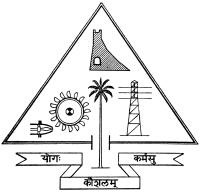
\includegraphics[scale=.8]{image/2.jpg}
% \end{figure}

% \vspace{0.7cm}
% \fontsize{14}{14}\selectfont
% \textbf{\centering CERTIFICATE}\\

% \vspace{0.5cm}
% \fontsize{12}{12}\selectfont
% \noindent
% \textit{This is to certify that the mini project titled } \textbf{\MakeUppercase{"AI Based Form Filling Assistant using Document Intelligence"}} \textit{is a bonafide work done by} \textbf{GOPIKA K (TCR24MCA-2033)} \textit{under my supervision and guidance, and is submitted in October 2025 in partial fulfillment of the requirements for the award of the Degree of Master of Computer Applications from APJ Abdul Kalam Technological University (KTU).}

% \vspace*{2.2cm}

% % \noindent
% % \begin{tabular}{p{5.2cm} p{5.2cm} p{5.2cm}}
% % \centering \textbf{Prof. Soumya Chandran} & \centering \textbf{Prof. Sreejith V.P.} & \centering \textbf{Dr. Sminesh C N} \\
% % \centering Project Guide 
% % \centering Project Coordinator  \\

% \vspace*{2 cm}
% \noindent{
% 	\begin{tabular}{p{4cm}cp{7cm}}
%         Prof.~ ~Soumia~Chandran~M&\hspace{1.5cm}Prof. Sreejith V P&\hspace{1.5cm}Dr. Sminesh C N\\
	      
% 		\textbf{Project Guide} &  \hspace{1.5cm} \textbf{Project Coordinator} &  \hspace{2cm}  \textbf{HOD} \\\\\\
	
% 		Place : THRISSUR & \hfill\\
% 		Date : 10-10-2025  &   \\\\\\
% 	\end{tabular}
% }

% \newpage

\justifying
\thispagestyle{empty}
\vspace*{0.5cm}
\fontsize{13}{13}\selectfont
\centering{\MakeUppercase{\textbf{DEPARTMENT OF COMPUTER APPLICATIONS}}} \\
\centering{\MakeUppercase{\textbf{GOVERNMENT ENGINEERING COLLEGE, THRISSUR}}} \\
\centering{\MakeUppercase{THRISSUR, KERALA STATE, PIN 680009 }} \\
\fontsize{12}{12}\selectfont
\vspace*{0.5cm}
\begin{figure}[ht]
{\centering {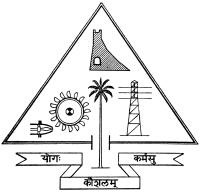
\includegraphics[scale=.8]{image/2.jpg}}\par}
\end{figure}
\vspace{0.7cm}
\fontsize{14}{14}\selectfont
\textbf{\centering{CERTIFICATE}}\\
\justify
\vspace{0.5cm}
\fontsize{12}{12}\selectfont
\textit{This is to certify that the mini project titled }
\textbf{\MakeUppercase{``RustAudit AI: Intra-Procedural Graph-Based
Semantic Analysis and Multi-Dimensional Software Quality Assessment for Rust"}}
\textit{is a bonafide work done by} \textbf{SOORAJ V}  \textbf{(TCR25MCA-2050)}
\textit{under my supervision and guidance, and is submitted in November 2026 in partial fulfillment of the requirements for the award of the Degree of Master of Computer Applications from APJ Abdul Kalam Technological University (KTU).}}
\\
\vspace*{2 cm}

\noindent



\hspace*{-0.8cm}
\noindent
\begin{tabular*}{\textwidth}{@{}l@{\extracolsep{\fill}}c@{\extracolsep{\fill}}r@{}}

Prof. Raseek C & Prof. Sreejith V P & Dr. Sminesh C N \\
\textbf{Project Guide} & \textbf{Project Coordinator} & \textbf{HOD} \\[2em]

Place : Thrissur & & \\
Date : 31-11-2026 & & \\

\end{tabular*}

\newpage
%\chapter*{DECLARATION}
I hereby declare that the main project named, \textbf{\MakeUppercase{AI-POWERED CODE DOCUMENT GENERATOR}}, is my own work and that, to the best of my knowledge and belief, it contains no material previously published by another person nor material which has been accepted for the award of any other degree or course of the university or any other institute of higher learning, except where due acknowledgment and reference has been made in the text.

\vspace{2cm}

\noindent
\begin{tabular*}{\textwidth}{@{\extracolsep{\fill}} l r}
Place : Thrissur & \textbf{ARYA K A} \\
Date : 31-03-2026 & \textbf{(TCR24MCA-2020)} \\
\end{tabular*}

\newpage
%% \chapter*{\rm \large \bf ACKNOWLEDGEMENT}
% \par\hspace{1.5cm}I would like to thank  Department of Computer Application, GEC Thrissur, for giving me this opportunity to pursue this project and successfully complete it.

% \par
% \hspace{1cm}I am highly indebted to our head of the department \textbf{Dr. Sminesh C N}, for his guidance and constant supervision as well as providing necessary information regarding the project and also for his support in completing the project.
% \par
% \hspace{1cm}I express my heart-felt gratitude to my project guide \textbf{Prof. Soumia Chandran}, for her committed guidance, valuable suggestions, constructive
% criticisms and precious time that she invested throughout the work.
% \par

%  \hspace{1cm} I \hspace{0.2cm}express\hspace{0.2cm} my\hspace{0.2cm} heart-felt\hspace{0.2cm} gratitude\hspace{0.2cm} to project coordinator\hspace{0.2cm} \textbf{Prof. Sreejith V P}, for her committed guidance as well as providing necessary information regarding the project, and also for her support in completing the project.

% \par
% \hspace{1cm}I sincerely thank all other faculties of MCA department for guiding me through the processes involved in the project.
% \newpage

\chapter*{\rm \large \bf ACKNOWLEDGEMENT}
\par\hspace{0.5cm}
\begin{justify}

\hspace{0.5cm}I would like to thank  Department of Computer Application, GEC Thrissur, for giving me this opportunity to pursue this project and successfully comple-te it.
\end{justify}

\begin{justify}

\hspace{0.5cm}I am highly indebted to our head of the department \textbf{Dr. Sminesh C N}, for his guidance and constant supervision as well as providing necessary information regarding the project and also for his support in completing the project. 
\end{justify}

\begin{justify}

\hspace{0.5cm}I express my heartfelt gratitude to my project guide \textbf{Prof. Sreejith V P}, for his committed guidance, valuable suggestions, constructive
criticisms and precious time that he invested throughout the work.
\end{justify}

\begin{justify}

\hspace{0.5cm}I express my heartfelt gratitude to project coordinator \textbf{Prof. Raseek C}, for his committed guidance as well as providing necessary information regarding the project, and also for his support in completing the project.
\end{justify}

\begin{justify}
    
\hspace{0.5cm}I sincerely thank all other faculties of MCA department for guiding me through the processes involved in the project.
\end{justify}

\newpage
\chapter*{\rm \large \bf ABSTRACT}
\vspace{3.0mm}
\begin{justify}

\hspace{0.5cm}Rust has emerged as a prominent systems programming language due to its strong guarantees of memory safety, concurrency, and high-performance execution. Despite these compile-time advantages, the operational quality of Rust applications remains highly dependent on localized developer implementation practices, including fine-grained ownership boundaries, micro-allocation behaviors, and loop safety mechanics. Existing static analysis ecosystems operate primarily on linear token patterns, providing fragmented, rule-based diagnostic alerts devoid of contextual reasoning regarding localized lifecycle mutations. Furthermore, current infrastructure tools lack the cross-layer evaluation models necessary to reason about how a localized memory allocation anti-pattern simultaneously degrades performance and code maintainability indicators inside a single subroutine body.
\par This paper presents RustAuditAI, an intra-procedural software quality intelligence framework that performs multi-dimensional semantic graph analysis bounded within individual Rust functions. The proposed system parses localized function syntax and constructs deep, interconnected semantic abstractions, including functional ASTs, localized CFGs, and dedicated FLOGs. By executing specialized traversal algorithms across this localized Code Property Graph structure, RustAuditAI unifies structural metrics with semantic analysis across four primary quality vectors: memory safety verification, code execution complexity, localized resource density, and defensive security. These analysis vectors are dynamically synthesized via a weighted valuation model to compute a standardized Rust Quality Index (RQI) representing localized code health. Bounded by the deterministic structural properties of the generated semantic graphs, an explainable recommendation engine generates context-aware, human-interpretable refactoring suggestions that specify the underlying structural degradation paths and estimate the quantitative execution optimizations achieved through more idiomatic Rust idioms.
\end{justify}
\end{spacing}


\pagestyle{plain}
\tableofcontents

\newpage
\addcontentsline{toc}{chapter}{List of Figures}
%\listoffigures
\newpage
%\addcontentsline{toc}{chapter}{List of Tables}
 %\listoftables
% \newpage] introduced LayoutLM, a pre-trained model that integrates
%\addcontentsline{toc}{chapter}{List of Algorithms}
%\listofalgorithms
\newpage
\clearpage
\chapter*{List of Abbreviations}
\addcontentsline{toc}{chapter}{List of Abbreviations}

\begin{center}
\renewcommand{\arraystretch}{1.4}
\begin{tabular}{p{1.8cm}cp{10cm}}

AI         & -- & Artificial Intelligence \\
API        & -- & Application Programming Interface \\
AST        & -- & Abstract Syntax Tree \\
BART       & -- & Bidirectional and Auto-Regressive Transformers \\
BLEU       & -- & Bilingual Evaluation Understudy \\
CD        & -- & Continous Integration \\
CI         & -- & Continous Deployment \\
CSS        & -- & Cascading Style Sheets \\
DFD        & -- & Data Flow Diagram \\
GPT        & -- & Generative Pre-trained Transformer \\
HTML       & -- & HyperText Markup Language \\
IDE        & -- & Integrated Development Environment \\
LLM        & -- & Large Language Model \\
METEOR     & -- & Metric for Evaluation of Translation with Explicit Ordering \\
Q/A        & -- & Question and Answer \\
REST API & -- & Representational State Transfer Application Programming Interface \\
RoBERTa    & -- & Robustly Optimized BERT Approach \\
ROUGE      & -- & Recall-Oriented Understudy for Gisting Evaluation \\
T5         & -- & Text-to-Text Transfer Transformer \\
URL        & -- & Uniform Resource Locator \\
UTF-8      & -- & 8-bit Unicode Transformation Format \\
VS Code    & -- & Visual Studio Code \\

\end{tabular}
\end{center}
\newpage

\pagenumbering{arabic}


\fontsize{12}{12}\selectfont	
\pagestyle{fancy}
\begin{spacing}{1.5}
\justifying 
%Start of chapters
\patchcmd{\chapter}{\thispagestyle{plain}}{\thispagestyle{fancy}}{}

\chapter{INTRODUCTION}
\patchcmd{\chapter}{\thispagestyle{plain}}{\thispagestyle{fancy}}{}

\hspace{0.5 cm}
In the contemporary computing landscape, systems programming languages form the bedrock of mission-critical infrastructure, including operating system kernels, cloud hypervisors, browser engines, and high-performance embedded networks. Historically, these low-level architectural layers were written exclusively in C or C++, exposing them to persistent categories of memory-safety exploitation vectors, such as buffer overflows, use-after-free anomalies, and dangling pointer dereferences. The emergence of the Rust programming language has redefined this domain by enforcing strict compile-time safety guarantees. Through a mathematically rigorous ownership model, affine type systems, and strict borrow checking boundaries, Rust eliminates traditional memory corruption bugs at compile time without the execution overhead of a runtime garbage collector.
\par However, the compile-time guarantees of Rust do not inherently ensure high-quality, secure, or operationally efficient software. While the compiler prevents fatal undefined behavior, human developers frequently struggle to adapt to the language's demanding structural constraints. This friction leads to widespread structural design flaws and anti-patterns inside individual subroutines. Developers routinely fight the borrow checker by over-relying on expensive runtime allocations, introducing redundant memory movements via excessive \textbf{.clone()} invocations, writing high-cyclomatic branching logic, or misusing \textbf{unsafe} code blocks to bypass compiler checks for localized optimizations.
\newpage
\par In contemporary DevSecOps ecosystems, identifying these quality bottlenecks is severely limited by a fragmented toolchain. Software teams must maintain multiple independent code inspection platforms: running \textbf{Clippy} for localized syntactic style lints, executing \textbf{cargo-audit} to detect known dependency advisory records, and using separate dynamic profilers to locate execution overhead. This disjointed execution path yields disconnected, plain-text diagnostic outputs that fail to communicate correlations among software dimensions. Traditional lint tools operate through linear token pattern-matching checks, completely lacking the contextual reasoning required to trace how a localized memory micro-allocation flaw simultaneously degrades performance and maintainability scores within a specific function body. 

\par To fundamentally resolve these structural challenges, this project introduces RustAuditAI, a novel, intra-procedural software quality intelligence framework that performs multi-dimensional semantic graph analysis bounded within individual Rust subroutines. Rather than executing shallow line-by-line checks over plain source code, the system ingests localized function syntax and constructs an advanced intermediate abstraction layer. Using the language compiler frontend, the framework builds a unified Code Property Graph (CPG) structure consisting of functional Abstract Syntax Trees (ASTs), localized Control Flow Graphs (CFGs), and a specialized, domain-specific Function-Level Ownership Graph (FLOG) that explicitly traces variable lifecycles, borrows, and structural move mutations. 

\par By executing graph-traversal slicing techniques over this multi-layered architectural representation, RustAuditAI unifies formal software engineering metrics with deep semantic analysis across four core analytical dimensions: memory safety verification, code execution complexity, localized resource density, and defensive security profiling. The quantitative indicators extracted from these dimensions are dynamically evaluated using a weighted linear matrix to compute a standardized Rust Quality Index (RQI)—a transparent, interpretable metric ranging from 0 to 100 that unifies localized code health into a single operational score.

\par To bridge the gap between automated detection and developer comprehension, RustAuditAI couples this deterministic graph infrastructure with an explainable artificial intelligence (XAI) interface driven by a Large Language Model (LLM). Bounded strictly by the structural properties of the generated semantic graphs, the system generates context-aware, human-interpretable refactoring insights. Instead of displaying abstract rule flags, the framework outputs detailed natural language reasoning explaining the underlying root cause of structural degradation, mapping the associated data propagation paths, and predicting the exact percentage of performance optimization achieved through idiomatic Rust alternatives. Finally, the system includes a self-contained visual engine that generates side-by-side behavioral diffs and highlighted execution graphs, providing an intuitive, user-controlled patch validation mechanism. By embedding RustAuditAI into software engineering lifecycles, developers can eliminate fragmented lint barriers, enforce rigorous software engineering standards, and maintain optimal performance parameters inside modern systems software.

\chapter{LITERATURE REVIEW}
\hspace{0.5cm}
The evaluation of software quality metrics and vulnerability localization models remains a core research frontier within software engineering and program security ecosystems. Historically, code analysis strategies have been split into two primary areas: rule-based static application security testing (SAST) and learning-based deep representation networks. While each methodology provides standalone analytical value, both exhibit significant design limitations when applied to the unique structural constraints and execution paradigms of the Rust programming language.

Traditional static analysis toolsets, exemplified by industry standard engines such as Fortify and SonarQube, rely heavily on deterministic pattern matching, text regex scanning, and pre-formulated rule databases to capture insecure code constructs. In the context of the Rust programming ecosystem, this paradigm is executed by the official compiler linter, Clippy, which relies on predefined abstract syntax checks to flag unidiomatic expressions. While highly effective at identifying shallow formatting irregularities or basic syntactic variations, these tools fall short when assessing deep logical vulnerabilities or cross-layer behavioral bottlenecks. Because linear token-matching mechanisms lack comprehensive data-flow tracking, they often produce high false-positive rates, miss complex structural defects that span conditional execution pathways, and fail to provide developers with actionable architectural reasoning.

To overcome the challenges of syntax-dependent code checking, compiler research has shifted toward structural graph abstractions that capture program behavior independently of source text. The foundational breakthrough in this domain was established by Yamaguchi et al. (2014), who formalized the concept of the Code Property Graph (CPG). By merging three distinct compiler representations—the grammatical Abstract Syntax Tree (AST), the execution-path-bound Control Flow Graph (CFG), and the data-dependence-tracking Program Dependence Graph (PDG)—into a single queryable graph database framework, the CPG transformed static analysis into a graph traversal problem. Tools built on this paradigm, such as the open-source analyzer \textbf{Joern}, allow security engineers to trace complex data propagation flows from input sources to vulnerable operation sinks. However, these traditional graph-based approaches remain strictly structural and deterministic. Their accuracy depends entirely on manual query development using specialized domain languages, leaving them unable to adapt to novel, context-dependent architectural flaws. Furthermore, classical CPG models are optimized for C/C++ memory models and lack the specialized semantic nodes needed to reason about Rust’s unique ownership, move, and reference borrowing rules.

Concurrently, the integration of deep learning and Natural Language Processing (NLP) has led to the development of massive transformer architectures trained on vast code corpora. Pre-trained language models for code, such as CodeBERT and GraphCodeBERT, have demonstrated strong capabilities across diverse software tasks, including vulnerability classification, defect prediction, and code summarization. Despite these advances, pure deep learning models face severe limitations when operating directly on raw high-level source code. As highlighted by Chakraborty et al. (2022) in their evaluation "\textit{Deep Learning Based Vulnerability Detection: Are We There Yet?}", token-based language models often lack true compiler-level comprehension. They are highly sensitive to superficial syntax modifications, variable renaming, and coding styles, which leads to unpredictable accuracy drops and high false-negative rates when processing subtle logic errors.

Building upon these foundational advancements, RustAuditAI introduces a highly specialized, intra-procedural software quality intelligence framework designed to address the unique complexities of the Rust language ecosystem. While existing literature focuses heavily on binary vulnerability detection or syntax-focused parsing, this project shifts the paradigm toward a multi-dimensional quality assessment engine. By extending the classical Code Property Graph with a custom Function-Level Ownership Graph (FLOG), the framework maps Rust's precise variable lifetimes and move metrics into queryable graph spaces. By feeding these structural graph contexts into state-of-the-art reasoning layers, RustAuditAI unifies deterministic software engineering formulas (such as McCabe’s Cyclomatic Complexity) with context-aware, explainable AI recommendation streams. This integration delivers an actionable, mathematically grounded, and developer-friendly code intelligence tool tailored for modern secure systems development.

\chapter{ENVIRONMENTAL STUDY}

\hspace{0.5cm}
This chapter outlines the hardware and software configuration environments required to successfully implement, deploy, and execute the RustAuditAI system. It details the platform constraints, compiler front-end parser utilities, language inference tools, and graph visualization libraries that form the underlying stack of the multi-dimensional software quality intelligence pipeline.

\section{System Configuration}
\hspace{0.5cm}
The operational environment for RustAuditAI spans specific physical computing architectures and virtual software execution layers designed to handle high-fidelity abstract syntax parsing and local model inference workflows efficiently.

\subsection{Hardware Requirements}
\hspace{0.5cm}
The hardware requirements outline the minimum resources necessary to operate the system. These resources are crucial for performing code analysis, processing tasks and running machine learning operations.

The key hardware requirements are detailed as follows:


\begin{itemize}
\item \textbf{Processor}: Intel\textsuperscript{\textregistered} Core\textsuperscript{\texttrademark} i5 Processor / AMD Ryzen\textsuperscript{\texttrademark} 5 Processor or higher, to efficiently handle code processing tasks.

\item \textbf{Memory}: Minimum 8 GB RAM, to ensure smooth execution of analysis and model operations.

\item \textbf{Storage}: 50 GB of free disk space, for storing code files and generated outputs.
\end{itemize}

\subsection{Software Requirements}
\hspace{0.5cm}
The requirements for software specify the necessary platforms, languages and libraries that will be used in running the system. The use of these tools, activities like parsing, integration and documentation become easy. Compatibility assurance is relevant to ensure that the various components of the system communicate effectively. 


The key software requirements are detailed as follows:
\begin{itemize}
    \item \textbf{Operating System}: Linux distribution (Ubuntu 22.04 LTS or later recommended), macOS Sequoia, or Microsoft Windows 11 configured with Windows Subsystem for Linux (WSL2).
    
    \item \textbf{Primary Implementation Platforms}: Python runtime environment version 3.11.x or later, alongside the native Rust compiler toolchain (rustc and cargo engine package utility version $\ge$ 1.75).
    
    \item \textbf{Version Control System}: Git open-source distributed source pipeline control suite.
    
    \item \textbf{Artificial Intelligence Interface Model}: Access token credentials for the centralized Groq inference platform API cluster utilizing the LLaMA-3.3-70B instruction-tuned model parameter footprint.
\end{itemize}

\subsection{Software Requirements for Development}
\hspace{0.5cm}Besides the execution specifications, some indispensable are the tools for development, testing and maintenance. They assist in writing and debugging programs, as well as managing the code appropriately. Besides, the tools help in maintaining versions and assembling different systems together. 

The key development software requirements for development are detailed as follows:
\begin{itemize}
    \item \textbf{Operating System}: Windows 10, Ubuntu 20.04 LTS or macOS, ensuring cross-platform compatibility.
    
    \item \textbf{Back End}: Python 3.8 or later, serving as the core implementation language.
    
    \item \textbf{IDE Used}: Visual Studio Code, Antigravity IDE used for development and debugging tasks.
    
    \item \textbf{Version Control}: Git open-source distributed source pipeline control suite.
    
    \item \textbf{Development Tools and Frameworks}:
    \begin{itemize}
        \item \textbf{syn crate:} Specialized parsing framework utilized to read and decode token streams into explicit Rust abstract syntax trees (ASTs).
        \item \textbf{quote and proc-macro2 crates:} To transform structured AST tokens back into compiler-valid syntactic elements for analysis slicing.
        \item \textbf{Pydantic crate/library:} Tasked with parsing and structurally enforcing input/output JSON schemas coming from the text reasoning layers.
        \item \textbf{NetworkX library suite:} Deployed as the core runtime graph data structure layout utility to handle localized nodes, edges, and path traversals for the Function-Level Ownership Graph (FLOG).
        \item \textbf{Requests or Httpx engine packages:} Configured to manage safe, asynchronous connectivity protocols with cloud API endpoints.
        \item \textbf{Rich text layout library:} Configured to parse code diagnostics into interactive terminal layout screens.
    \end{itemize}
\end{itemize}
\section{Software Specification}
\hspace{0.5cm}The following section provides a detailed description of different software components and technologies that are used to design the system under discussion. This is because each of the software components performs specific tasks that shall be useful when analyzing the code and preparing the documentation. Each software component is made to perform particular operations that are useful in code analysis and documentation preparation and the use of technologies is meant to ensure a smooth integration process. 

\subsection{Python 3.8}
\hspace{0.5cm}
Python functions as the primary execution coordinator for RustAuditAI. It orchestrates the lifecycle of the static analysis pipeline, handling file validation, initiating external compilation checks, managing the graph data structures inside NetworkX, and routing extracted semantic data vectors to the remote inference gateways. Python’s mature data structure packages and rich reporting wrappers make it the ideal platform to bind the deterministic compiler graph layers with the downstream explainable text engines.

\subsection{Rust Toolchain(syn and cargo)}
\hspace{0.5cm}
The native Rust ecosystem acts as the foundational parsing source engine for this framework. The syn crate acts as a robust compiler front-end parser that ingests standard .rs file text strings and decodes them into fully structural Abstract Syntax Trees (ASTs). This component preserves localized code expressions, statement mappings, control constructs, and identifier paths. By relying on syn, RustAuditAI gains direct access to precise compiler-level representations of function scopes without requiring fully compiled intermediate binary builds, establishing the raw data foundation for the custom Ownership and Control Flow graphs.

\subsection{The Function-Level Ownership Graph (FLOG) Engine}
\hspace{0.5cm}
The FLOG Engine is a core domain-specific novelty created for this project using the NetworkX library. It translates abstract code definitions into explicit variable lifecycle tracking paths. It generates nodes representing allocation footprints (such as local references, box vectors, and variable re-bindings) interconnected by edges detailing ownership rules (such as moves, mutable borrows, or immutable aliases). This custom data structure enables the static analysis engine to perform deep intra-procedural lifecycle evaluations, mathematically identifying code flaws like allocation leaks or excessive cloning behaviors before execution.

\subsection{Git}
\hspace{0.5cm}
Git is used as the version control system for analyzing the structure of the repository and obtaining historical information regarding the code. This allows the system to work with entire projects by cloning repositories from remote sites, which eliminates manual uploading of separate files. Information at the commit level is also available, for example, for the production of documentation, such as a list of the latest changes. 

\par This would enable the system to be able to identify the different types of changes through commits, thus being able to identify development patterns and get knowledge on how the code is being changed over time. All this would lead to context being better understood, thereby adding a layer of value to the kind of document that is being generated. Other than source code repositories, the system would also allow local source code directories to ensure flexibility with the various types of input sources. 

\subsection{NetworkX}
\hspace{0.5cm}
It is used to create and analyze the graphs representing the relationships, function calls and dependencies in the code. NetworkX helps the system to model the code structure as a directed graph, where the functions are represented as nodes and the interactions are represented as edges. This allows the system to understand important parts of the program code, such as the starting point, recursion and any dependencies. The use of graph-based analysis increases the understanding of how the code operates. Additionally, the system uses graph analysis to perform complex evaluations of the code, enabling a better understanding of its critical components.

\subsection{Explainable AI (XAI) Module}
\hspace{0.5cm}
The Explainable AI module improves operational transparency by turning raw, numeric quality checks into clear, natural language recommendations. Rather than printing standard compiler diagnostics or raw text warning codes, this component uses structured semantic properties to explain why an expression violates best practices. It explicitly documents the data path where a variable bottleneck emerges and includes structural feedback explaining how a suggested update modifies execution dependencies. This detailed explanation turns abstract graph diagnostics into educational, highly actionable refactoring advice for developers.

\subsection{Visualization Support}
\hspace{0.5cm}
The visualization engine translates internal graph structures into self-contained HTML reports featuring interactive Control Flow Graphs (CFGs) and variable lifecycle grids. Built without external layout software dependencies, it provides custom visual highlights along vulnerable or inefficient execution pathways inside a function body. By showing a side-by-side behavioral comparison between original and proposed code structures, the module enables developers to trace attack vectors or performance bottlenecks visually, improving system transparency and patch management.
\chapter{SYSTEM ANALYSIS}

\par
\hspace{0.5cm}
The practice of performing systems analysis in a technical development scenario focuses on identifying the most effective way to solve a relevant problem—such as detecting vulnerabilities and software quality bottlenecks in source code. Before initiating the development of such a system, project stakeholders, including researchers or student developers, formulate a project proposal and present it to the concerned academic or institutional authority for review and approval.

\par A structured system inquiry in this context involves evaluating the current challenges developers face in identifying and securing their code, with the goal of enhancing these processes using advanced tools like language parsers and large language models (LLMs). System analysis is used to break down the problem, identify key objectives—such as code transformation, analysis, and vulnerability classification—and ensure all modules work cohesively to deliver accurate and helpful insights to the developer or learner using the system.

\section{Requirements Analysis}
\hspace{0.5cm}
Requirement analysis is a crucial phase in the software development life cycle that focuses on identifying, documenting, and analyzing the functional and technical needs of a system before design and implementation. For the proposed RustAuditAI project, which aims to perform intra-procedural software quality intelligence, vulnerability detection, and explainable patch generation within individual Rust functions, this phase plays a vital role in defining the system's scope and expected behavior.

The primary requirement of the system is to support source code blocks written in the Rust programming language. Individual functions must be parsed into a structured abstract form using compiler-level front-ends, specifically the syn crate ecosystem. This compiler-level syntax extraction enables language-idiom validation and forms the foundation for consistent, intra-procedural data-flow and lifetime tracking without requiring full workspace compilation binaries.

Another key requirement is the integration of Large Language Models for semantic code reasoning and software quality analysis. The system must be capable of extracting localized graph properties from the Abstract Syntax Tree (AST), Control Flow Graph (CFG), and Function-Level Ownership Graph (FLOG), and providing them as structured context inputs to LLMs for identifying safety defects, allocation bottlenecks, and logical vulnerabilities. In addition to detection, the system is required to generate natural-language explanations using Explainable AI (XAI) techniques, ensuring that developers understand the root cause, execution flow, and structural impact of each detected quality degradation pattern.

The system must also support automatic patch generation, where secure and optimized code fixes are produced for identified function flaws. These fixes should be presented in a clear old-versus-new diff format to allow developers to review, apply, or refine the suggested patches. Furthermore, visualization support is required to generate interactive, self-contained functional Control Flow Graphs that visually illustrate the propagation of variables, resource allocations, and the specific structural branches leading to code degradation.

In addition to functional requirements, several non-functional requirements must be satisfied. The system should provide highly efficient intra-procedural analysis with rapid execution times suitable for active development loops. It must maintain strict determinism in its mathematical scoring engine and be extensible enough to incorporate additional performance or safety criteria in the future. Usability is also a critical requirement, with metrics and reports designed to be clear, educational, and developer-friendly.

This requirement analysis ensures that the RustAuditAI system is aligned with its intended objectives and provides a reliable foundation for subsequent system design, implementation, and evaluation.

\section{Existing System}
\hspace{0.5cm}
Existing systems and tools for Rust code verification and vulnerability detection are mainly designed to identify known insecure coding patterns or isolated syntax deviations. Most of these systems rely on traditional static analysis techniques, strict compiler rule sets, or independent linters. While such approaches are effective for enforcing foundational language rules, they often struggle to capture multi-dimensional structural correlations, subtle performance bottlenecks, and logic-level design flaws inside subroutines. Furthermore, many existing tools operate in complete isolation and do not provide a unified framework for measuring overall software quality from an architectural perspective.

Another major limitation of existing systems is their lack of contextual explainability and automated remediation support. Most tools focus only on detection and produce plain-text warnings without clearly explaining the broader architectural cause, execution overhead, or optimization path. As a result, developers must manually interpret the results and implement fixes, which increases debugging effort and code complexity. Some of the widely known systems include:
\begin{itemize}
    \item \textbf{Clippy:} Clippy is the default, official collection of lints for the Rust programming language. It operates by scanning source code files for the presence of known unidiomatic patterns, styling deviations, and minor logical errors. It is lightweight and fast, making it highly suitable for enforcement during standard compilation routines. However, Clippy relies heavily on syntax pattern matching over the compiler's Abstract Syntax Tree, which limits its ability to dynamically correlate disparate software attributes. This often results in isolated text warnings that lack explanatory depth regarding how a specific variable change cascades to affect performance and maintainability metrics simultaneously. Additionally, Clippy is restricted strictly to syntactic rule validation and does not offer context-aware natural language explanations or automated patch comparison dashboards.
    \item \textbf{cargo-audit:} Developed by the Rust Secure Code Working Group, cargo-audit focuses entirely on supply-chain security and dependency vulnerability scanning. It operates by evaluating a project's dependency manifest (Cargo.lock) against the official Rust Advisory Database to detect crates with publicly disclosed vulnerabilities (CVEs). While essential for dependency management, cargo-audit is blind to the internal code logic written by the developer. It cannot inspect function bodies, analyze variable lifetimes, or track inefficient resource allocation densities within subroutines. Moreover, cargo-audit primarily functions as a binary checker (reporting the presence or absence of vulnerable dependencies) and provides no utility for custom code refactoring, structural visualization, or automated code optimization.
    \item \textbf{Joern:} Joern is an advanced open-source static analysis engine that compiles source code into a Code Property Graph (CPG), blending abstract syntax trees, control-flow graphs, and data-flow graphs into a unified graph structure. This graph abstraction allows for deep semantic queries over program dependencies. However, Joern's accuracy relies entirely on manually formulated queries written in a specialized domain-specific language, creating a steep learning curve and restricting its utility to expert security auditors. Furthermore, Joern's standard graph schema is optimized for C/C++ pointer behaviors and entirely lacks dedicated node types to model Rust’s unique compile-time ownership semantics, lifetime variables, and borrow checking restrictions. It also fails to integrate large language models for explainable reasoning or interactive patch generation.
\end{itemize}

\section{Limitations of Existing System}
\hspace{0.5cm}
Though there is access to documentation technology, the existing systems have the following drawbacks:

\begin{itemize}
\item \textbf{Dependence on Isolated Syntactic Signatures:} Most existing Rust analysis tools rely on rigid, syntax-based signature matching to flag unidiomatic code blocks. These signatures check for precise token patterns and fail to reason about the underlying semantic intent of the subroutine. Consequently, such systems struggle to identify custom logical inefficiencies or context-dependent resource bottlenecks that do not match a pre-configured linter rule.

\item \textbf{Fragmented and Compartmentalized Outputs:} Current tools operate as completely independent utilities, forcing developers to manage separate workflows for code styling, security checking, and profiling. This fragmentation prevents the cross-layer correlation of data; for instance, an entry-level developer cannot see how an over-reliance on deep memory copies (.clone()) to bypass a compiler warning directly degrades performance while simultaneously complicating the function’s long-term maintainability.

\item \textbf{Lack of Standardized Software Quality Metrics:} The existing ecosystem produces discrete lists of diagnostic warnings and errors rather than providing a unified evaluation of overall code health. The absence of a standardized, multi-dimensional metric specific to Rust makes it difficult for project managers and developers to easily measure, track, or prioritize structural improvements over the lifecycle of a subroutine.

\item \textbf{Absence of Explainable Context and Educational Feedback:} Legacy tools generate brief error messages or static diagnostic links that state what code line is triggering an alert, but omit a comprehensive explanation of why it degrades software quality. This missing reasoning path slows down verification and triage, offering very little educational value to developers who are trying to learn how to write more idiomatic Rust code.

\item \textbf{Lack of Automated and Interactive Remediation Support:} Current tools stop at alerting the developer to a potential violation and offer no active assistance in correcting it. The responsibility of researching, writing, and validating an alternative implementation remains entirely manual. This manual remediation process is time-consuming and error-prone, highlighting the clear need for systems that synthesize, display, and apply validated fixes automatically under developer control
\end{itemize}

\section{Proposed System}
\hspace{0.5cm}
The proposed system, RustAuditAI, is designed to provide a comprehensive, intra-procedural software quality intelligence framework by integrating compiler-level graph abstractions with the advanced reasoning and context-aware capabilities of Large Language Models (LLMs). By combining deterministic program structures with language-tuned reasoning layers, the system achieves highly precise, context-aware, and multi-dimensional quality assessment bounded strictly within individual Rust functions. Unlike conventional linters or rule-based tools that rely on isolated syntax patterns, this system constructs an internal, multi-layered Code Property Graph tailored explicitly for Rust’s unique execution semantics, exposing variable states, localized branching structures, and micro-allocation operations in a unified format.

The system translates localized function blocks into structured semantic definitions, creating functional Abstract Syntax Trees (ASTs), localized Control Flow Graphs (CFGs), and a dedicated Function-Level Ownership Graph (FLOG) that explicitly maps variable lifetimes, borrows, and ownership re-bindings. These representations serve as the structured input data for an LLM specialized in code intelligence, enabling the framework to evaluate complex code behaviors that traditional tools miss. The proposed architecture consists of the following core modules:
\begin{itemize}
    \item \textbf{Syntax Parsing \& Graph Generation Module:} This module accepts target Rust function code text and utilizes the compiler frontend syn crate to extract an abstract syntax tree. The module maps localized code expressions, conditional paths, and identifier references into an interconnected graph layer. By standardizing raw text into an active graph structure, it builds the explicit functional blueprint needed for multi-vector inspection.
    \item \textbf{The FLOG Engine Module:} Once the baseline syntax structures are built, this specialized engine generates the Function-Level Ownership Graph. It defines nodes for every localized variable allocation and reference type, connecting them with explicit semantic edges that track lifetime bounds, move variables, and borrow mutations. This maps Rust's precise compiler rules directly into a mathematical graph layout.
    \item \textbf{Multi-Dimensional Metric Computation Engine:} This component simultaneously navigates the generated graphs across four distinct quality vectors: Safety (tracking unsafe blocks and borrow mechanics), Performance (measuring allocation and clone density), Maintainability (calculating McCabe's Cyclomatic Complexity), and Security (identifying hazardous API traits). It applies formal software engineering formulas to produce normalized scores for each vector.
    \item \textbf{The RQI Synthesis Module:} This engine aggregates the independent criteria scores using a weighted valuation matrix to compute the unified Rust Quality Index (RQI) on a scale from 0 to 100. It utilizes a dynamic penalty matrix where a critical safety violation or illegal alias automatically triggers non-linear deductions that lower adjacent quality vectors, providing a true mathematical reflection of localized code health.
    \item \textbf{Explainable AI (XAI) \& Patch Synthesis Module:} Upon identifying code flaws, this module feeds the structured graph anomalies into the LLM interface, bounding its reasoning strictly within the deterministic facts of our graph. The module generates targeted patch options in an old-versus-new diff format alongside clear natural language reasoning. It explains the exact cause of code degradation, outlines the refactoring strategy, and quantifies the expected performance improvements to guide the developer toward optimal programming practices.
\end{itemize}

\section{Advantages of Proposed System}
\hspace{0.5cm}
The proposed software quality intelligence framework offers several key advantages that enhance the static analysis process and provide significant value to systems developers and educational institutions alike. By combining specialized ownership graphs with bounded LLM reasoning layers, the system ensures highly precise, unified, and actionable code quality evaluations.

\begin{itemize}
\item Unified Multi-Dimensional Evaluation: Instead of forcing developers to jump between fragmented linter and security binaries, the system evaluates code health across four critical engineering vectors simultaneously, mapping the results onto a singular dashboard.
\item Rust-Specific Ownership Mapping: The inclusion of a dedicated Function-Level Ownership Graph (FLOG) bridges a massive gap in academic literature by providing an explicit graph structure to track variable moves, lifetimes, and borrow distributions inside function scopes.
\item Mathematical and Deterministic Scoring: The creation of the Rust Quality Index (RQI) provides a standardized, objective indicator (0–100) grounded in established formulas like Cyclomatic Complexity, allowing team leads to easily track code quality evolution.
\item Explainable, Context-Aware AI Remediation: By constraining the LLM within the deterministic facts of the semantic graphs, the system completely prevents AI hallucinations, producing high-fidelity, educational explanations that detail the precise root causes of code degradation.
\item Interactive, User-Controlled Patching: The framework displays proposed alternative code snippets in a visual side-by-side diff layout, ensuring that all modifications remain fully under developer control and preventing unauthorized codebase revisions.
\item Highly Optimized Performance Loop: Because the framework is strictly scoped to intra-procedural analysis (evaluating a single function at a time), it circumvents the immense processing bottlenecks of cross-workspace points-to analysis, delivering rapid feedback suitable for agile development workflows.
\end{itemize}

\section{Functional Requirements}
\hspace{0.5cm}
The proposed system is designed to perform intra-procedural software quality analysis, vulnerability detection, and explainable patch generation within individual Rust functions by leveraging advanced Abstract Syntax Trees (ASTs), localized Control Flow Graphs (CFGs), Function-Level Ownership Graphs (FLOGs), and Large Language Models (LLMs). The functional requirements outline all expected behaviors, user interactions, and internal system capabilities in detail. 

\subsection{Source Code Input and Upload}
\hspace{0.5cm}
The system shall allow users to input or upload isolated Rust source code blocks or function snippets through a dedicated interface. Target files can be uploaded or pasted directly as individual .rs files or function code segments. The system shall validate uploaded data to ensure it contains syntactically valid Rust structural declarations before initiating subsequent compilation checks. The system shall provide immediate, descriptive error messages for unsupported file formats, empty payloads, or major syntax compilation failures. The system shall not accept files with unsupported extensions or text that does not resolve into a standard language function block.

\subsection{Language Identification and Preprocessing}
\hspace{0.5cm}
Upon submission, the system shall automatically detect the language parameters and map the input text directly to the native Rust analysis pipeline.The system shall isolate the structural bounds of the specific subroutine or function scope, filtering out external module variables or global package definitions to enforce strict intra-procedural analysis boundaries.  Based on the detected function format, the system shall prepare the code token stream for direct conversion into an intermediate graph abstraction layer using compiler-level parsing crates.

\subsection{Graph Abstraction and Representation Generation}
\hspace{0.5cm}
The system shall successfu
lly generate a multi-layered Code Property Graph abstraction from the function source code using the compiler frontend syn crate backend. The generated graph representation must:
\begin{itemize}
    \item Extract a functional Abstract Syntax Tree (AST) mapping localized syntax declarations and statement properties.
    \item Construct a localized Control Flow Graph (CFG) mapping basic block nodes and conditional execution pathways.
    \item Build a domain-specific Function-Level Ownership Graph (FLOG) that explicitly models variable lifetimes, references, borrows, and move operations. 
\end{itemize} 
The system shall verify successful graph construction and report errors if compilation errors or structural anomalies break graph creation boundaries.The system shall not proceed with subsequent LLM analysis routines if initial graph abstraction generation fails.

\subsection{Vulnerability and Quality Vector Detection using LLM}
\hspace{0.5cm}
The system shall parse the constructed semantic graphs to extract localized graph contexts and variable interaction summaries representing internal function behaviors. The system shall submit these graph properties as structured context inputs into the LLM interface to perform semantic reasoning across multiple evaluation layers. The LLM reasoning engine shall identify:
\begin{itemize}
    \item Unsafe and memory-safety anomalies, including unvalidated pointer arithmetic, unchecked unsafe scopes, or invalid reference lifecycles.
    \item Performance and resource efficiency defects, including excessive or redundant .clone() operations, unnecessary heap allocations, or inefficient iterator tracking loops.
    \item Maintainability flaws, including overly complex conditional loops, high line-count expressions, or long nested branch layouts.
    \item Defensive security bugs, including data validation flaws or reliance on deprecated or hazardous API traits. 
\end{itemize} 
The system shall classify and tag every identified flaw with a dedicated severity metric (low, medium, high, critical), exact functional statement location, and targeted CWE tracking identification index.

\subsection{Rust Quality Index (RQI) Report Generation}
\hspace{0.5cm}
Once semantic graph processing is completed, the system shall execute its mathematical scoring engines to compile a comprehensive Rust Quality Index (RQI) report.
The generated report shall display:
\begin{itemize}
    \item A unified, composite RQI health score ranging from 0 to 100 based on weighted evaluation matrices.
    \item Individual score metrics for each of the independent evaluation vectors (Safety, Performance, Maintainability, Security).
    \item Non-linear deduction logging displaying how severe single anomalies dynamically penalize adjacent vectors.
    \item Technical descriptions, impact scenarios, and specific mitigation options for every identified flaw.
\end{itemize}
The completed quality reports shall be exportable as highly readable, self-contained dashboard files or PDF documents for static project review.

\subsection{Patch Generation, Validation, and Version Management}
\hspace{0.5cm}
After code flaws are flagged, the system shall visually highlight the exact functional statement lines inside the workspace interface. The system shall invoke the LLM-based patch synthesis engine to output one or multiple secure, compilable refactoring candidates for the identified vulnerabilities.
Each generated patch recommendation must include:
\begin{itemize}
\item An optimized, refactored function source code snippet replacing the original vulnerable block.
\item Natural language explanations detailing the structural mechanics of the fix.
\item Estimated performance improvements, resource savings, or index optimization impacts.
\end{itemize}
The system shall present all refactoring recommendations to the user in a side-by-side comparison format, ensuring that code updates remain completely user-controlled. Upon user confirmation and approval of a recommended patch, The original function code block is replaced by the secure version in the current workspace. The framework automatically switches to the patched version as the active codebase. The system regenerates the corresponding AST, CFG, and FLOG graph models to verify that the target issue has been successfully resolved.

\subsection{Code Revision and Patch Control}
\hspace{0.5cm}
The system shall maintain a thorough intra-procedural revision database tracking every approved modification layer. Each revision entry shall store a full historical copy of the preceding code structure, the specific patch details, and an exact timestamp identifier. The system shall provide an accessible rollback/revert feature, enabling users to instantly reset the function back to any earlier version state. Upon executing a rollback, the function code is immediately restored, and its original graph abstractions and metrics are re-calculated and displayed.

\subsection{Visualization of Subroutine Graph Abstractions}
The system shall provide a built-in visualization interface displaying high-fidelity interactive models of the Control Flow Graph (CFG) and the Function-Level Ownership Graph (FLOG). During the initial assessment phase, inefficient branching execution paths, excessive allocation nodes, and vulnerable instruction sequences shall be highlighted inside the graph interface. During patch validation, the interface shall render side-by-side graph models showing the old structure vs. the new optimized abstraction layout to visually demonstrate path removal and optimization.

\subsection{Error Handling}
The system shall provide meaningful error messages for validation failures, unsupported syntax, parser errors, or timeout exceptions during API communication. The framework shall handle complex, large subroutines gracefully, logging nested parsing exceptions without breaking the workspace database or corrupting active data states.

\section{Non-Functional Requirements}
\hspace{0.5cm}
The non-functional requirements specify quality attributes for the syst . They ensure that the systems output is accurate, consistent and that it functions effectively and remains user-friendly. The non-functional requirements specify the quality attributes for the system to ensure that it is effective, u r-friendly and produces the right output and that it emphasizes on scalable, usability and reliability that underpins implementing a robust and practical AI-powered documentation solution. 

\subsection{Performance}
\hspace{0.5cm}
The system must execute all operational tasks—including syntax tree generation, FLOG construction, metrics extraction, LLM context evaluation, and report compilation—efficiently. Because the platform is strictly restricted to an intra-procedural execution scope, response latencies during static analysis loops should remain low enough to facilitate an interactive development loop without performance bottlenecks.

\subsection{Usability}
\hspace{0.5cm}
The user interface should prioritize clarity, accessibility, and clean design for both learners and developers. The dashboard must present quality indicators clearly, utilizing interactive code panels, synchronized side-by-side patch diff layouts, and visual graph displays that make complex ownership mutations and refactoring steps easy to trace.

\subsection{Accuracy and Reliability}
\hspace{0.5cm}
System reliability is maintained through rigorous, deterministic graph metrics combined with transparent patch validation loops. The framework must accurately evaluate structural and control flows, ensuring that the calculated metrics reflect the true state of the function scope. The platform preserves source stability by ensuring that no code modifications are ever executed automatically without explicit developer consent.

\subsection{Security and Confidentiality}
\hspace{0.5cm}
All user-submitted function code blocks are analyzed in an isolated, secure execution environment. The platform ensures that no uploaded source material or intermediate graph databases are permanently stored or exposed after analysis is complete. Proper input validation and sandboxing are enforced throughout the pipeline to protect the tool from malicious execution exploits.

\subsection{Maintainability and Extensibility}
\hspace{0.5cm}
The framework must feature a highly modular architecture that cleanly separates the parsing front-end, the metric calculation module, the LLM reasoning interface, and the reporting dashboard. This modular configuration allows developers to easily update assessment rules, swap underlying text inference models, or integrate the framework into continuous deployment workflows without requiring an architectural overhaul.

\subsection{Explainability}
All code quality evaluations and vulnerability detections must be justified with natural language explanations detailing the underlying structural root causes. Every suggested patch must include structured reasoning that clearly defines the safety or performance enhancements achieved, allowing developers to understand both the cause of the issue and the exact structural effect of the proposed solution.

\subsection{User-Controlled Patch Management}
The application must guarantee that patch validation remains entirely under user control. Developers must be provided with side-by-side textual code comparisons and structural graph differences, enabling them to evaluate, accept, or discard recommendations as needed before any modifications are committed to the file system.

\section{Feasibility Study}
\hspace{0.5cm}
A feasibility study examines a proposed system to determine its viability, impact on operations, ability to meet user needs, and cost-effectiveness. While any project might seem achievable given unlimited time and resources, it is essential to assess feasibility early to ensure practicality and success. Systems that integrate emerging technologies, such as advanced language compilers and large language models, require such evaluation to anticipate implementation challenges, technical risks, and operational constraints.
In the case of the proposed RustAuditAI framework, a feasibility study helps evaluate whether the intra-procedural analysis system can fulfill technical metrics, work efficiently within target workflows, and deliver practical value for software quality engineering. The study is divided into three sections:

\subsection{Technical Feasibility}
\hspace{0.5cm}
The technical feasibility of RustAuditAI is grounded in the architectural choice to restrict code parsing to an intra-procedural scope using mature compiler utilities. By utilizing the robust syn crate, the frontend can reliably transform raw function text into structured Abstract Syntax Trees without the immense compute overhead required for full cross-workspace compilation. The integration of the NetworkX library allows for high-performance generation and traversal of the custom Function-Level Ownership Graph (FLOG), accurately tracking variables, lifetimes, and borrows.
The language reasoning layers are handled via secure API connections to highly optimized instruction-tuned models like LLaMA-3.3-70B, which provide fast text inference speeds and low latency. The local visualization engines utilize clean HTML and CSS formatting, avoiding dependencies on heavyweight external layout frameworks. Because all underlying parsing libraries, graph models, and API interfaces are well-supported and extensively documented, the construction of the system is highly feasible within standard computing environments without specialized hardware acceleration.

\subsection{Operational Feasibility}
\hspace{0.5cm}
Operational feasibility evaluates whether the system can function efficiently in the intended environment and satisfy user requirements. RustAuditAI is explicitly structured to introduce minimal disruption into active development loops, operating as a lightweight, interactive function-level assistant. By focusing on localized routines, it provides immediate quality metrics, RQI logs, and visual graph trees that help developers rapidly inspect code logic.
The split dashboard—showing side-by-side code diffs, actionable explanations, and patch histories—is designed to be highly accessible to developers with varying security and systems expertise. The platform is equally effective for project managers tracking quality trends and for students learning idiomatic systems programming concepts. Therefore, the tool is highly feasible from an operational perspective across both educational and industry environments.

\subsection{Economical Feasibility}
\hspace{0.5cm}
Economic feasibility assesses whether the benefits of the system justify the associated costs. The primary development expenditures involve minor computing resources for local graph generation and processing standard cloud API tokens for text reasoning queries. Relying on open-source compiler crates like syn and standard hardware configurations drastically lowers upfront infrastructure costs compared to building proprietary analysis engines.
By automatically evaluating software metrics, flagging allocation vulnerabilities, and providing instant refactoring patches under developer control, the framework significantly reduces the time and cost associated with manual code optimization and security code remediation. This automated approach delivers long-term productivity gains and reduces potential runtime vulnerabilities, making RustAuditAI highly cost-effective and economically feasible for academic research and deployment pipelines.

% \subsection{Error Handling}
% Invalid inputs, unsupported files, or analysis failures shall be
% detected and communicated to the user through appropriate error
% messages.

% \subsection{Data Security}
% The system shall process source code locally and shall not permanently
% store or transmit user code without authorization, ensuring data
% privacy and security.

% \section{Feasibility Study}
% \hspace{0.5cm}A feasibility study evaluates the practicality of implementing the
% proposed system in terms of technical, operational, and economic
% factors. This assessment ensures that the system can be developed using
% available resources within reasonable constraints.

% \subsection{Technical Feasibility}
% \hspace{0.5cm}The system utilizes widely supported technologies such as Python,
% AST-based parsers, vector databases, and large language models. The
% computational requirements are moderate and can be satisfied using
% standard personal computing environments, making the system technically
% feasible.

% \subsection{Operational Feasibility}
% \hspace{0.5cm}The system is designed to require minimal user interaction and technical
% expertise. Users only need to provide a source code location to obtain
% generated documentation, making the system operationally feasible for
% students, developers, and academic users.

% \subsection{Economical Feasibility}
% \hspace{0.5cm}The system is developed using open-source tools and libraries. No
% specialized hardware or licensed software is required, making the
% proposed solution cost-effective and economically feasible.

%\chapter{SYSTEM DESIGN}
\hspace{0.5cm}
The design of the AI-Powered Code Documentation Generator is elaborated on in this chapter, emphasizing the organization and structure of system components and the travel of the source code through the pipeline process stages of language identification, feature extraction, AST analysis and the LLM engine until accurate and structured documentation is eventually generated. A modular design approach is used, where every component has an individual purpose in the entire system. This chapter also discusses how the modules interact with each other and how the data flow from the input (source code) to the output (documentation). 
\section{System Architecture}
\hspace{0.5cm}
As depicted in Figure 5.1, the architecture of the proposed system represents an AI-driven pipeline for automated code documentation. The process begins when the user provides source code, either by uploading a file or supplying a repository URL. Initially, the input is analyzed by the Language Detection Module to determine the programming language, ensuring that subsequent parsing is accurate. Following this, the system conducts two parallel processes: the Text Feature Extraction Module captures surface-level code features, while the AST Analysis Module generates a structured representation of the code’s components.

\par The AST output is then sent to the Graph Building Module, where a graph is constructed with nodes representing functions or classes and edges representing relationships such as function calls and dependencies. The outputs from the Text Analysis Module, AST Module and Graph Building Module are then combined in the Feature Fusion Module to produce a comprehensive representation that integrates the textual, structural and relational aspects of the code.
\par This integrated representation is then fed into the LLM Module, which produces human-readable documentation. The Documentation Module organizes this content into various document formats and delivers the finalized documentation to the user.
\newline


\FloatBarrier
\begin{figure}[htbp]
    \centering
    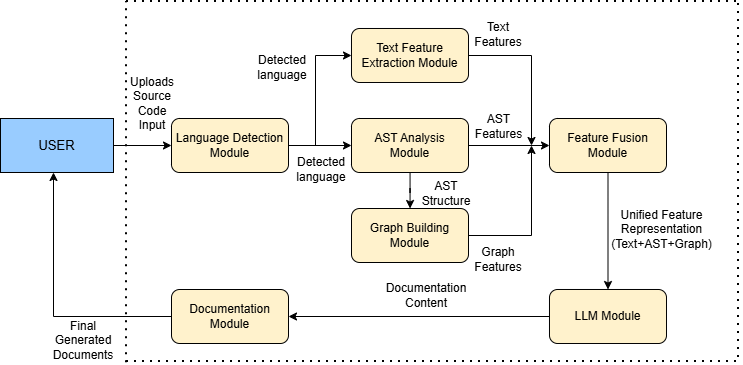
\includegraphics[width=\textwidth]{tex/Untitled Diagram-Page-2.drawio (3).png}
    \caption{Architecture Diagram of the AI-Powered Code Documentation Generator.}
    \label{fig:architecture}
\end{figure}
\FloatBarrier



\section{Data Flow Diagram (DFD)}
\hspace{0.5cm}Figures 5.2 and 5.3 illustrate the data flow diagrams of the proposed system, showing the complete movement of data throughout the automated code documentation generation process.
\subsection{DFD Level 0}

\hspace{0.5cm}Figure 5.2 demonstrates the Level 0 Data Flow Diagram (DFD) of the AI-Powered Code Documentation Generator. The user provides source code to the system, which uses AST analysis to extract essential details such as functions, classes, imports and other relationships. Based on this extracted information, the AI generates structured documentation and delivers it to the user.
\hspace{0.3cm}
\FloatBarrier
\begin{figure}[h]
	\centering
	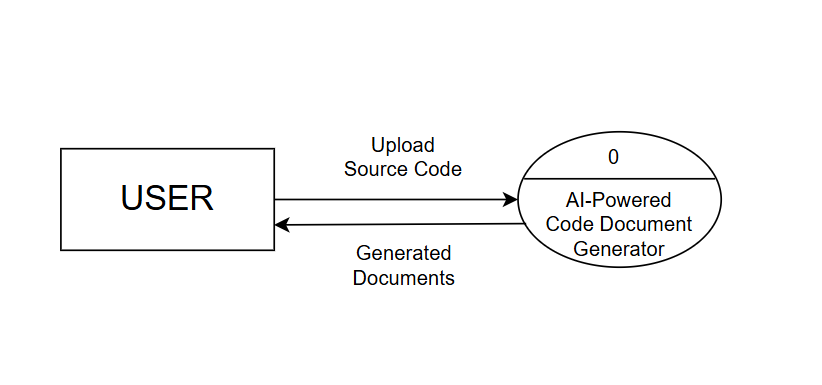
\includegraphics[scale=0.6]{tex/Screenshot 2026-04-13 101331.png}
	\caption{Data Flow Diagram Level 0.}
	\label{lvmh2}
\end{figure}
\subsection{DFD Level 1}


\hspace{0.5cm}Figure 5.3 presents the internal processing of the AI-Powered Code Document Generator as a Level 1 DFD. The process begins when the user uploads the source code and the Language Detection Module identifies the programming language based on the file extension. Once the language is detected, two parallel streams occur: the Text Feature Extraction Module extracts textual information and code metrics, generating text data, while the AST Extraction Module parses the code to create its abstract syntax tree, representing its structural organization. The AST is then passed to the Graph Feature Extraction Module to produce graph-based features capturing relationships among functions, classes and method calls. All features are merged in the Feature Fusion Module, which is subsequently processed by the LLM Engine (Ollama) to generate a natural language description of the source code. Finally, the Document Generation Module formats this output into structured documentation for the user.

\hspace{0.3cm}
\FloatBarrier
\begin{figure}[htbp]
    \centering
    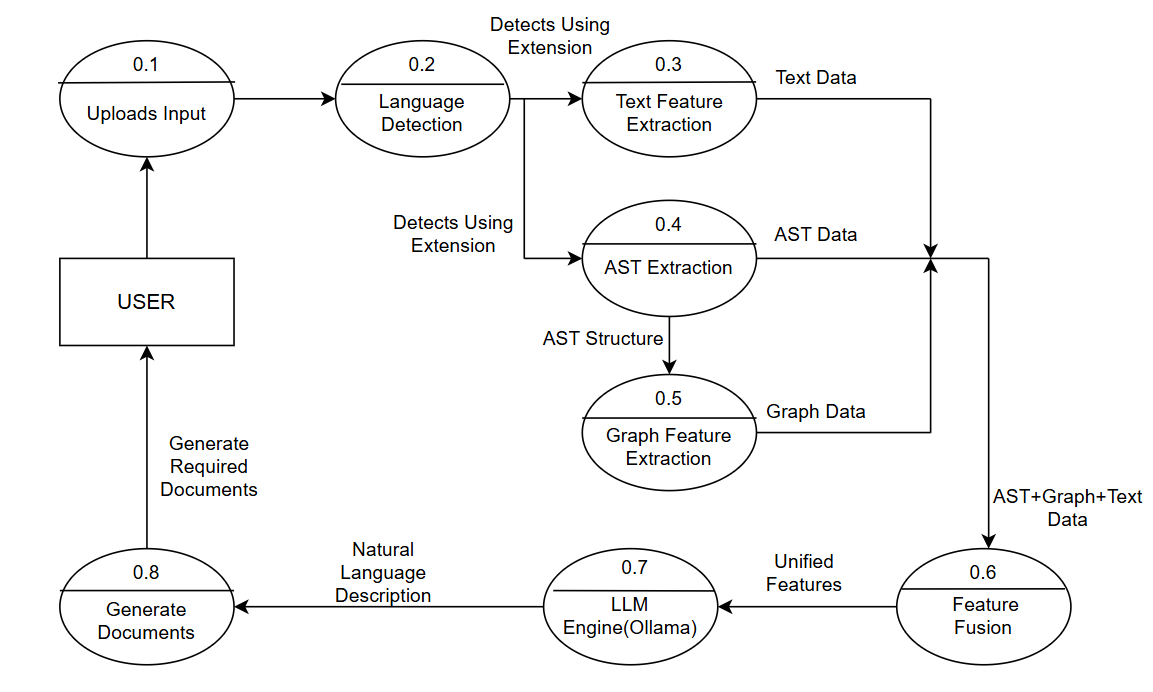
\includegraphics[width=\textwidth,keepaspectratio]{tex/Screenshot 2026-03-11 142330.png}
    \caption{Data Flow Diagram Level 1.}
    \label{fig:dfd1}
\end{figure}

\newpage


\section{List of Modules}
\hspace{0.5cm}
The AI-Powered Code Documentation Generator is composed of the following modules:
\begin{itemize}
    \item User Interface Module
    \item Language Detection Module
    \item Text Feature Extraction Module
    \item AST Analysis Module
    \item Graph Building Module
    \item Feature Fusion Module
  
    \item LLM Engine Module
    \item Documentation Output Module
\end{itemize}

\subsection{User Interface Module}
\hspace{0.5cm}
This module serves as the main interface between the user and the system. It allows users to provide source code files, project directories or repository URLs and access both the generated documentation and the results of intermediate analysis. The interface ensures smooth navigation through each step of the process, making the analysis workflow seamless for the user.

\subsection{Language Detection Module}
\hspace{0.5cm}
The Language Detection Module identifies the programming language of the uploaded source code by analyzing file extensions and syntax. This detected language guides the system in selecting the appropriate parsing strategies and analysis methods. Accurate identification ensures correct AST generation and feature extraction, allowing the system to efficiently process multi-language projects and improving overall flexibility and adaptability.

\subsection{Text Feature Extraction Module}
\hspace{0.5cm}
This module extracts text-based features from the source code, calculating metrics such as the number of lines, tokens, comments, identifiers and keywords. It also identifies import statements, revealing external libraries and dependencies used in the project. These features are critical for generating project-level documentation, including README files and technology stack summaries, providing a comprehensive overview of the codebase. The module operates independently of language-specific syntax, making it fast and lightweight.

\subsection{AST Analysis Module}
\hspace{0.5cm}
This module analyzes the structure of the source code using an AST. It provides detailed insights into the internal structure of the code by extracting classes, functions, parameters, return types, variables, imports and function calls. As a core module, it ensures accurate and meaningful documentation based on the code itself rather than assumptions. It also supports language-aware analysis to enhance extraction accuracy and efficiency.

\subsection{Graph Building Module}
\hspace{0.5cm}
This module constructs a semantic graph from the AST. Nodes represent code elements such as files, classes and functions, while edges indicate relationships like function calls, imports and inheritance. The graph provides a clear visualization of interactions among code components, illustrating data flow and module dependencies. It also supports deeper analysis, including the identification of recursion, unused functions and critical components.

\subsection{Feature Fusion Module}
\hspace{0.5cm}
This module integrates textual features, AST-based structural features and graph-based relational features. Textual features provide specific information, AST features detail the functionality of each component and graph features illustrate the relationships between components. By combining all these features, the system can generate more accurate and comprehensive documentation, ensuring that no information is lost during processing.

\subsection{LLM Engine Module}
\hspace{0.5cm}
This module uses a LLM to create human-readable documentation. The input to the module consists of feature summaries created from the AST, text and graph analysis. The model uses the structural and contextual information to create accurate documentation about the functionality of the code and the architecture of the system. This ensures the readability, accuracy and appropriateness of the created documentation. The level of detail in the documentation depends on the complexity of the input code.

\subsection{Documentation Output Module}
\hspace{0.5cm}
This module handles structuring the generated documentation in an organized layout, covering areas such as project overview, architecture, API documentation and module-level details. It ensures consistency in presentation, enhancing readability and usability. The documentation can be exported to formats like Markdown, making integration with existing development workflows easier and supporting efficient sharing and management.
\newline
\par In this chapter, the overall system design of the AI-Powered Code Documentation Generator is discussed, including the system architecture, the functionality of its various modules and the complete data flow. This design enables each module to process the source code independently while ensuring that the analysis and documentation generation proceed systematically and cohesively. With the system’s design and architecture established, the next chapter will cover the implementation aspects, detailing the development of each module and how they integrate to achieve the intended functionality.

%\chapter{SYSTEM IMPLEMENTATION}
\hspace{0.5cm}
The system implementation phase is aimed at realizing the AI-Powered Code Documentation Generator design. At this stage, full development occurs, including the implementation of all system modules, such as the code parser, structural feature extraction algorithm, semantic understanding algorithm and automatic documentation generator. Each module is developed and implemented independently, allowing developers to make changes or enhancements without affecting other modules. This approach ensures high scalability, as modifications and additions can be implemented easily while maintaining the integrity and efficiency of the system.
\section{Setup Development environment}
\hspace{0.5cm}The importance of having an efficient development environment cannot be ignored when implementing and executing the system. In the context of the current system, the VS Code editor is chosen as the development environment for its lightweight structure and easy integration with different tools. The backend is designed with the Python 3.8 language because of the numerous benefits that come with the use of this language when processing data and implementing machine learning algorithms. The HTML (HyperText Markup Language), CSS (Cascading Style Sheets) and JavaScript languages are used to implement the frontend of the system to make the interaction experience of the user more engaging. The backend server has been implemented using the Flask web framework, which helps in creating RESTful APIs for the smooth communication between the frontend and backend modules.
To support the implementation of various functionalities, the following Python libraries are installed and configured:\begin{itemize}
\item \textbf{Flask} -- This tool is used in constructing the backend server as well as the REST (Representational State Transfer) API endpoints. It manages all requests made by users, like uploading files. This too starts the code analysis and sends back the documentation that is created.

\item \textbf{Tree-sitter} -- This tool is used for parsing source code and converting it into ASTs, enabling accurate syntactic analysis for multiple programming languages. It divides the source code into structural elements such as functions, classes and other components.

\item \textbf{Tree-sitter-languages} -- This library provides built-in language support that extends Tree-sitter’s capabilities, allowing the system to support multiple programming languages such as Python, Java, JavaScript, C, C++, Go, Rust and Kotlin without the need for separate parser configurations for each language.

\item \textbf{Markdown} -- A Markdown library provides tools to parse, render and manipulate Markdown content programmatically.  
Such libraries support creating dynamic documentation, reports or web content from plain text. 
They simplify integrating Markdown-based documentation into automated systems and applications.

\item \textbf{Networkx} -- This tool is used to construct and analyze graph structures derived from the parsed code helping to achieve a deeper contextual understanding of the code.
\end{itemize}
\section{User Interface}
\hspace{0.5cm} The User Interface is built as a single-page application with HTML, CSS and JavaScript, enabling users to upload source code files, folders or even input a public Git repository URL. The User Interface supports three modes: Single File, Folder and Mixed.

\par The frontend sends a request to the \textit{/analyze} endpoint to communicate with the Flask-based backend. Once the request is received, the backend will process the input by calling the core function \textit{analyze\_path()}. This function will determine whether the input is a file, folder or Git URL and then route it to the appropriate analysis pipeline. If it is a Git URL, the repository will be cloned to a temporary directory and then cleaned up. If it is a local input, the function will directly call either the single-file analysis pipeline or the project-level analysis pipeline based on whether the path is pointing to a file or a directory.

\par The generated documentation will be displayed in the browser as formatted HTML using the marked.js library. Users will also be able to download the complete generated Markdown files as a ZIP package using the JSZip library.

\section{Language Detection}
\hspace{0.5cm}
The next step is to recognize the programming language of each uploaded source file based on its file extension. This is done by utilizing an extension-to-language mapping defined in \textit{language\_config.py}, which allows the system to support twelve programming languages including Python, Java, JavaScript, TypeScript, C, C++, Go, Rust, PHP, Ruby, Kotlin and C#.

\par During processing, the file extension is extracted from the file path, which is converted to lowercase for standardization purposes, as different operating systems have different capitalization standards. After that, the programming language is detected based on the predefined file extension mapping.

\par In order to ensure robustness, the unsupported file types will be skipped during the traversal of the folders. Also, empty files will be removed prior to the start of the analysis process. Moreover, the Git metadata directories such as \textit{.git} will be skipped during the traversal of the folders using the normalized paths where backslashes will be replaced with forward slashes in order to support both the Windows and Linux platforms, thus preventing the Git source code from being treated as source code.

\section{Text Feature Extraction}
\hspace{0.5cm}
In this stage, lightweight textual features are obtained from individual source files without reference to the AST, aiming to identify basic structural properties of the code. The features are calculated through text-based analysis in \textit{text\_features.py} without any reference to language parsing or grammar.

\par The function reads the source file in a safe manner with UTF (Unicode Transformation Format)-8 encoding and ignores decoding errors for robustness across different file types and legacy codebases. In case the file is invalid or cannot be read, an empty dictionary is returned.

\par The features that are extracted are the raw counts, which include the total number of lines, the total number of characters, the number of import statements, the number of class definitions and the number of function definitions. These features offer an overview of the source file.

\par These metrics are attached to every function record as a \textit{metrics} field. They help in the formation of the unified fused representation in the downstream modules.

\section{AST Analysis}
\hspace{0.5cm}
In this stage, structural information is obtained through structural feature extraction, where each source file is parsed to an AST with the help of the tree-sitter framework, facilitating precise analysis for all fourteen programming languages.

\par The entry point is \textit{tree\_sitter\_adapter.py} where the programming language is resolved based on the file extension, the source file is read in a safe manner with UTF-8 encoding and the parse tree is generated along with a source representation at the byte level to accurately extract the text within nodes. Node type names such as function definitions, class declarations and call expressions for different languages are read from \textit{language\_config.py} to ensure that the logic itself doesn’t have any explicit language checks.

\par The AST is processed in \textit{ast\_graph.py} with a two-pass strategy. The first pass traverses the entire AST tree structure to collect all the function names, class names and import symbols in the \texttt{known\_names} set. The \textit{known\_names} set will be used in the second pass of the AST traversal process to differentiate calls to functions defined within the project codebase from calls to external library code. The \textit{known\_names} set is supplemented with symbols obtained from all the files in the codebase in the global pre-pass in \textit{analyzer.py}.

\par The second pass carries out full per-function extraction. For a function, the system extracts the function's name, class membership, parameters, return type, internal function calls, external function calls, local variables and string literals. For function names, a four-strategy cascade is used to accommodate the different structural characteristics of programming languages. Most languages rely on a direct field lookup for function names, while the languages C and C++ rely on a declarator chain walk and a shallow identifier scan and a deep recursive scan serve as a fallback.

\par Although function calls are identified during this process, the caller-callee relation is not stored as a string. Rather, every identified internal call is directly added to the NetworkX graph by invoking \textit{graph.add\_edge()}. This graph is the sole source of all call relation data. The extracted function-level metadata is stored in the \textit{metadata} dictionary and passed to the next stage, Graph Analysis.


\section{Graph Analysis}
\hspace{0.5cm}
Within this stage, the semantic graph created during the AST traversal process is examined to determine higher-level structural information about the codebase. The graph is built using the NetworkX library, in which the nodes of the graph represent the functions and the edges represent the caller-callee relations. The graph is the single source of truth for all call relationship data, which means the data about the relations of the functions is not obtained from intermediate lists of strings or the AST.

\par The call relationships in the graph are obtained by using successor queries on the graph, where the outgoing edges on a function node directly provide the list of functions it calls. This method ensures consistency throughout the system and avoids the need for string parsing and redundant storage.

\par In addition to storing the relationships between the entities, the graph is used to find four different structural characteristics in the code. The entry points in the code are the set of functions that have no incoming edges but have outgoing edges; in other words, these are the functions that are never called by any other function in the code but start the calls themselves. The dead functions in the code are the set of functions that have neither incoming nor outgoing edges; in other words, these are the functions that are never called in the code and never start any calls either. A cross-file check is done before determining the dead or entry point functions in the code.

\par Direct recursion is identified through self-loop edges in the graph, where a function has an edge pointing back to itself. Mutual and chain recursion are detected using cycle detection algorithms, which identify groups of functions forming circular call chains of length greater than one. Critical functions are determined by ranking nodes based on their in-degree, where functions with a higher number of incoming edges are considered the most depended-upon in the codebase.
\par These features of the derived graphs are included in each function’s record and passed on to the Feature Fusion and Documentation Generation stages, which enrich the LLM prompt with architectural information that cannot be automatically inferred from the AST features.

\section{Feature Fusion}
\hspace{0.5cm}
At this stage, features extracted by the Text Feature Extraction, AST Analysis and Graph Analysis modules are integrated into a single structure for each function. This integration encompasses the structural, relational and contextual aspects of the code in a single structure, which is used by all the modules.

\par The fusion is achieved in \textit{analyzer.py} through the \textit{\_build\_record()} function, which constructs one record per function by combining three different sources of information. The information from the AST is used for the structural facts about each function, including its name, its membership in a class, parameters, return type, external calls, local variables, string literals and imports. The information from the graph is used for the relational facts, including the list of internal calls and the formatted caller-callee relationship strings, both of which are obtained directly from graph successor queries. The text features include the contextual metrics, including the raw counts used by the LLM..

% \par The graph acts as the single source of truth for all call relationship data throughout the fusion process. Rather than storing call relationships as strings during the AST walk, they are derived at record construction time by querying the graph, which eliminates redundancy and ensures that the relationships stored in the record always reflect the actual graph structure.

% \par The complete graph analysis result from \texttt{analyze\_graph()} is also embedded in each function record. This includes entry points, dead functions, direct recursion, mutual cycles, most critical functions, and the longest execution path — all of which are used in the documentation generation stage to provide architectural context to the LLM.

\par The resulting fused records are serialized into \textit{semantic\_records.json}, which is used as the persistent interface between the analysis pipeline and the module for generating the documentation.


\section{Documentation Generation}
\hspace{0.5cm}
The Documentation Generation Module uses the open-source LLM DeepSeek, which is hosted locally via Ollama, to create structured Markdown documentation from the integrated code records. The model is accessed via the Ollama HTTP API with a low temperature of 0.1 to ensure consistent and factually reliable outputs. The \textit{stream: false} parameter ensures that the complete response is returned as a single JSON (JavaScript Object Notation) payload, simplifying downstream processing.

\par For each function, a structured fact block is created from the fused record and passed into the LLM as a prompt. This fact block combines all three sources of features into one line of context.


\par All documents are generated in parallel by a \textit{ThreadPoolExecutor} with up to six concurrent workers, greatly improving the total generation time for large projects. If a document does not generate correctly, it will have a stub so that the pipeline always produces a complete output even in the presence of individual failures


\par The module produces four types of Markdown documentation artifacts per run of the analysis:
\begin{itemize}
\item \textbf{README.md} for project overview, description, tech stack, project structure, etc.
\item \textbf{architecture\_overview.md} for component responsibilities, data flow between files, module dependencies, etc.
\item \textbf{File-wise .md files} for file-wise information like import information, member variables, function intents, parameters, return types, function call relationships, entry points, dead code, recursion and cycles.
\item \textbf{recent\_changes.md} for displaying Git commit history with author information and message for every commit, if input is provided as a Git repository URL.
\end{itemize}

\par The implementation phase has been successfully completed to transform the proposed design into a fully functional form of the AI-Powered Code Document Generator. All the modules, ranging from language detection and AST parsing to graph analysis, feature fusion and LLM-based generation, have been implemented and integrated to function cohesively in a complete system. Since the system has been fully operational for a range of programming languages and input types, the discussion will move on to the evaluation stage. The next chapter will cover the results achieved by running the system on a range of projects and a discussion on the quality, accuracy, and completeness of the generated documentation.

% \begin{lstlisting}[language=python]
% from sentence_transformers import SentenceTransformer, util

% model = SentenceTransformer('all-MiniLM-L6-v2')

% def map_profile_to_form(profile, form_fields):
%     mapped = {}
%     for field, value in profile.items():
%         best_match = None
%         best_score = -1
%         for form_field in form_fields:
%             score = util.cos_sim(
%                 model.encode(field, convert_to_tensor=True),
%                 model.encode(form_field, convert_to_tensor=True)
%             )
%             if score > best_score:
%                 best_score = score
%                 best_match = form_field
%         mapped[best_match] = value
%     return mapped
% \end{lstlisting}

% \section{Form Auto-Filling}
% \hspace{0.3cm}
% The final mapped data is converted to JSON and sent to the frontend. 
% A JavaScript script runs on page load to automatically fill the form fields 
% with the extracted details.

% \begin{lstlisting}[language=javascript]
% <script>
%   const filledData = {{ final_form_data | tojson }};
%   window.onload = () => {
%     for (let key in filledData) {
%       const el = document.querySelector(`[name="${key}"]`);
%       if (el) el.value = filledData[key];
%     }
%   };
% </script>
% \end{lstlisting}


% \hspace{0.3cm} This module-based implementation ensures flexibility to add more document types in the future while keeping extraction accurate and rule-based.

% Thus, the system completes the pipeline: document upload $\rightarrow$ 
% text extraction (PDF-first, OCR for images if required)$\rightarrow$ field extraction $\rightarrow$ consolidation $\rightarrow$ 
% form field mapping $\rightarrow$ auto-filling.
%\chapter {RESULTS AND DISCUSSION}
\hspace{0.5cm}
This chapter presents and analyzes the results obtained from the proposed system, the AI-Powered Code Documentation Generator. The system was evaluated using source code files provided through two input methods: direct file uploads via the web interface and repository-based inputs through public Git URLs. This dual-mode testing ensured that the system was assessed under both isolated and real-world development scenarios.

The results demonstrate that the system is capable of effectively processing multi-language codebases and generating well-structured, coherent and contextually relevant documentation. By integrating techniques such as syntactic analysis, structural feature extraction and language model-based generation, the system successfully transforms raw source code into meaningful documentation. Overall, the observed outputs highlight the system’s reliability, scalability and practical applicability in automating documentation tasks across diverse programming environments..

\section{Results}
\hspace{0.5cm}The system was tested in different input modes to evaluate its functionality and output quality. The following figures illustrate the working of the system and the documentation generated at various stages.
\par The screenshot in Figure 7.1 displays the homepage of the AI-Powered Code Documentation Generator when in file upload mode. There are two modes in which a user can input the source code. These modes are Upload Files and Repository URL.
\vspace{1cm}
\FloatBarrier
\begin{figure}[h]
	\centering
	\fbox{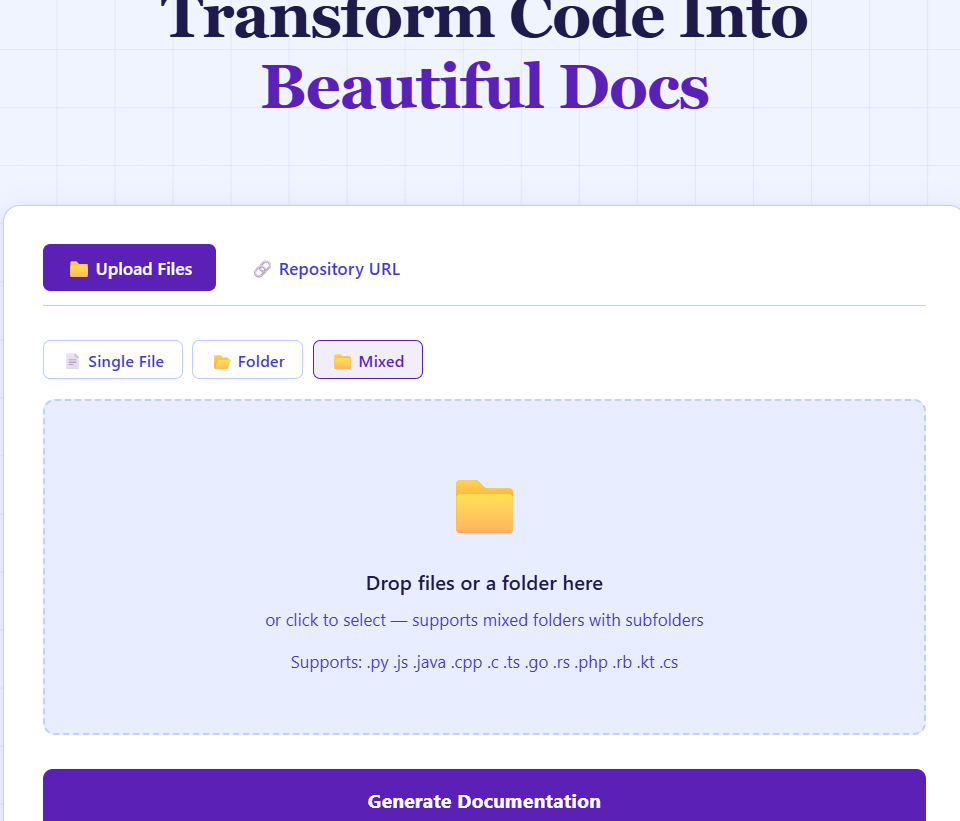
\includegraphics[width=0.6\textwidth]{tex/Screenshot 2026-04-14 215024.png}}
	\caption{Complete User Interface of the System.}
	\label{lvmh2}
\end{figure}
\FloatBarrier

\vspace{1cm}
\begin{figure}[h]
	\centering
	\fbox{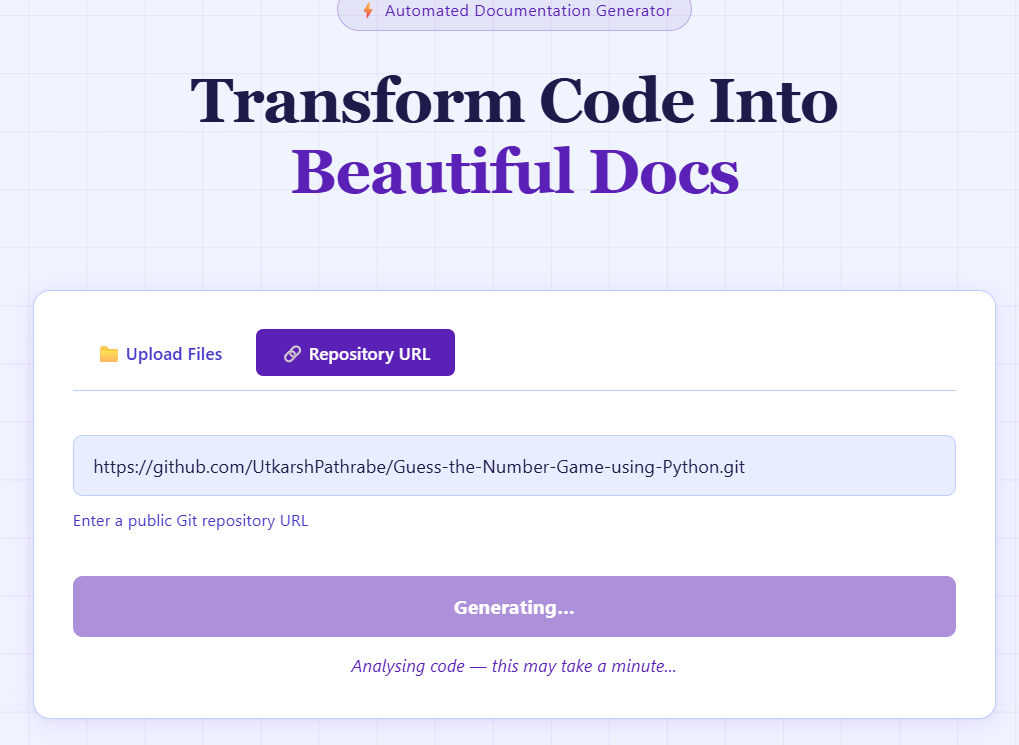
\includegraphics[width=0.6\textwidth]{tex/Screenshot 2026-04-16 072516.png}}
	\caption{Home Page – Repository URL Input Mode.}
	\label{lvmh2}
\end{figure}
\FloatBarrier

\par Figure 7.2 shows the User Interface (UI) for the homepage with the Repository URL mode selected. The user can provide the public git repository URL in the text box. The system then downloads the repository in a temporary directory and processes all the source files from the repository without the need to upload the files.

\vspace{1cm}
\FloatBarrier
\begin{figure}[h]
	\centering
	\fbox{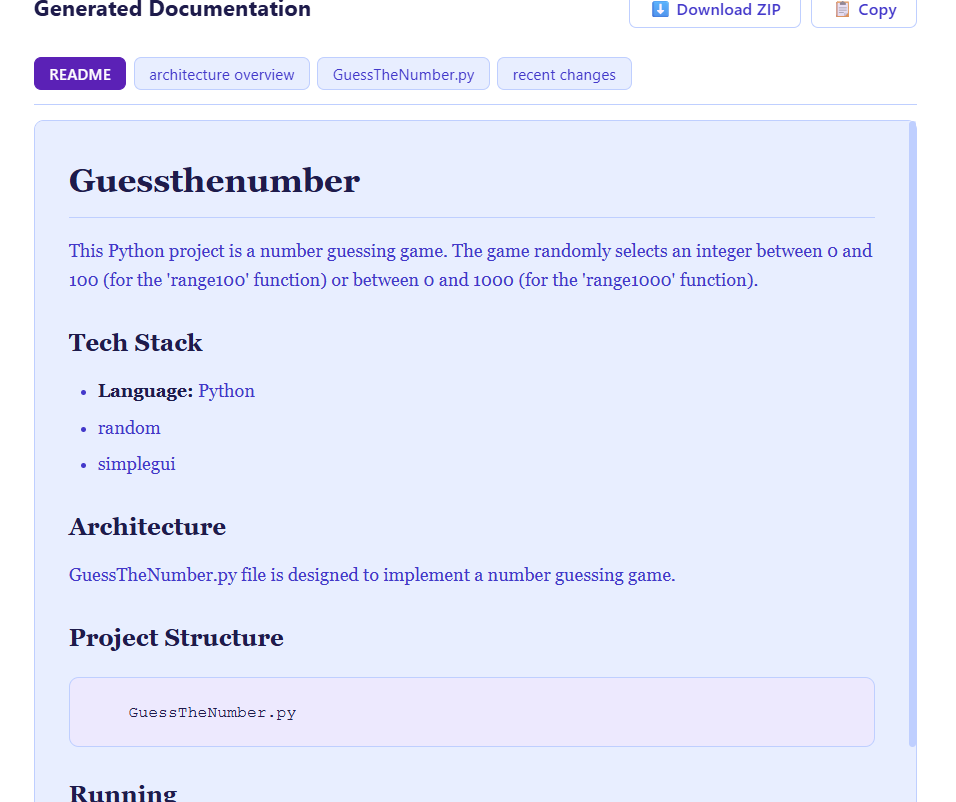
\includegraphics[width=0.6\textwidth]{tex/Screenshot 2026-04-16 073000.png}}
	\caption{README.md – Project Overview Output.}
	\label{lvmh2}
\end{figure}
\FloatBarrier

\par The system shows the README tab of the generated documentation output in Figure 7.3. It analyzes the repository and provides a project-level summary, including project description, technology stack, architecture summary, run instructions, and project structure.

\vspace{1cm}
\FloatBarrier
\begin{figure}[h]
	\centering
	\fbox{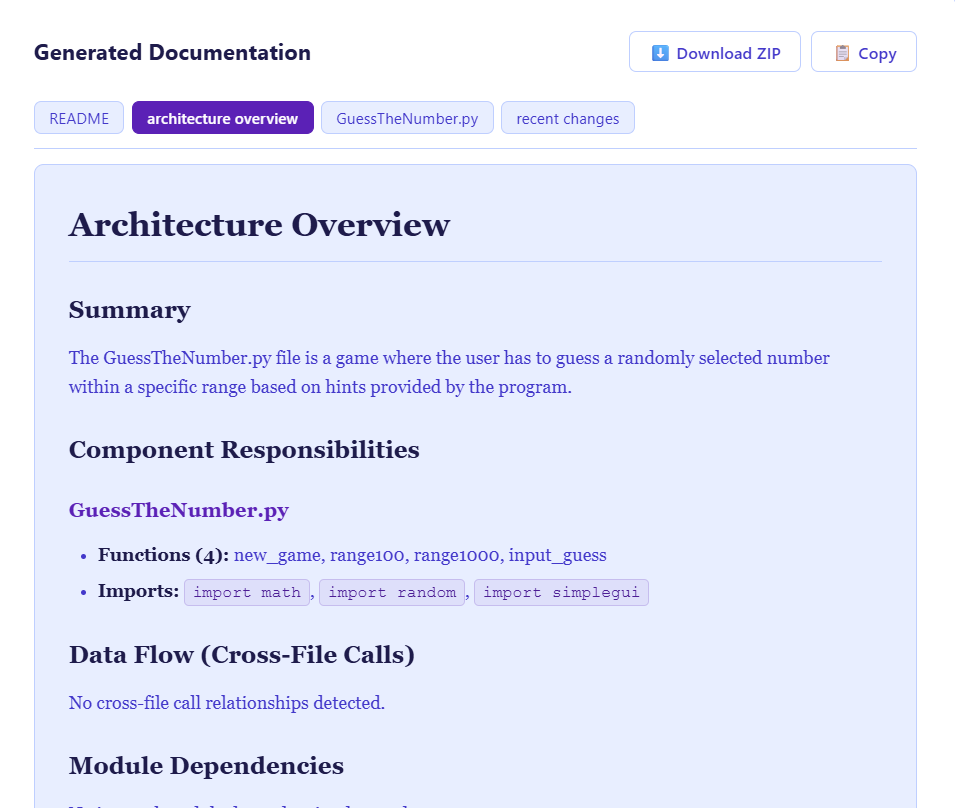
\includegraphics[width=0.6\textwidth]{tex/Screenshot 2026-04-16 073016.png}}
	\caption{architecture\_overview.md – Architectural Description Output.}
	\label{lvmh2}
\end{figure}
\FloatBarrier

\par Figure 7.4 shows the system displaying the Architecture Overview tab of the automatically generated documentation. The system generates a structured architectural description consisting of file-wise summary information, component responsibilities such as classes, functions, imports and fields, call relationships between files representing data flow and module dependencies from both import statements and function interactions.

\par Figure 7.5 shows the file-wise documentation generated for the application in Markdown format. Each file has its documentation with information like function intent, parameters, return values, function calls, local variables and internal call relationships, along with graph-based information like entry points, unused functions, dependencies and recursion information.

\vspace{1cm}
\FloatBarrier
\begin{figure}[h]
	\centering
	\fbox{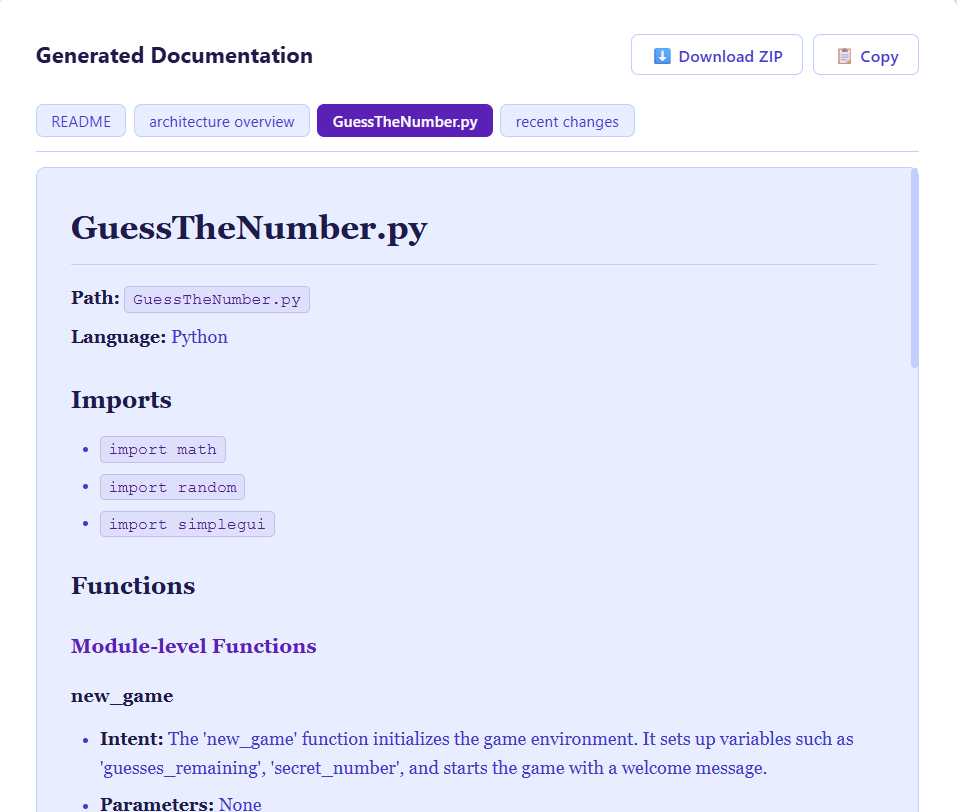
\includegraphics[width=0.6\textwidth]{tex/Screenshot 2026-04-16 073038.png}}
	\caption{File-wise .md Output.}
	\label{lvmh2}
\end{figure}
\FloatBarrier

\par Figure 7.6 shows the Recent Changes tab of the automatically generated documentation. The system has automatically collected the commit history from the Git repository and created a structured document named recent\_changes.md. This feature helps users easily track project updates and understand the evolution of the codebase over time.

\vspace{1cm}
\FloatBarrier
\begin{figure}[h]
	\centering
	\fbox{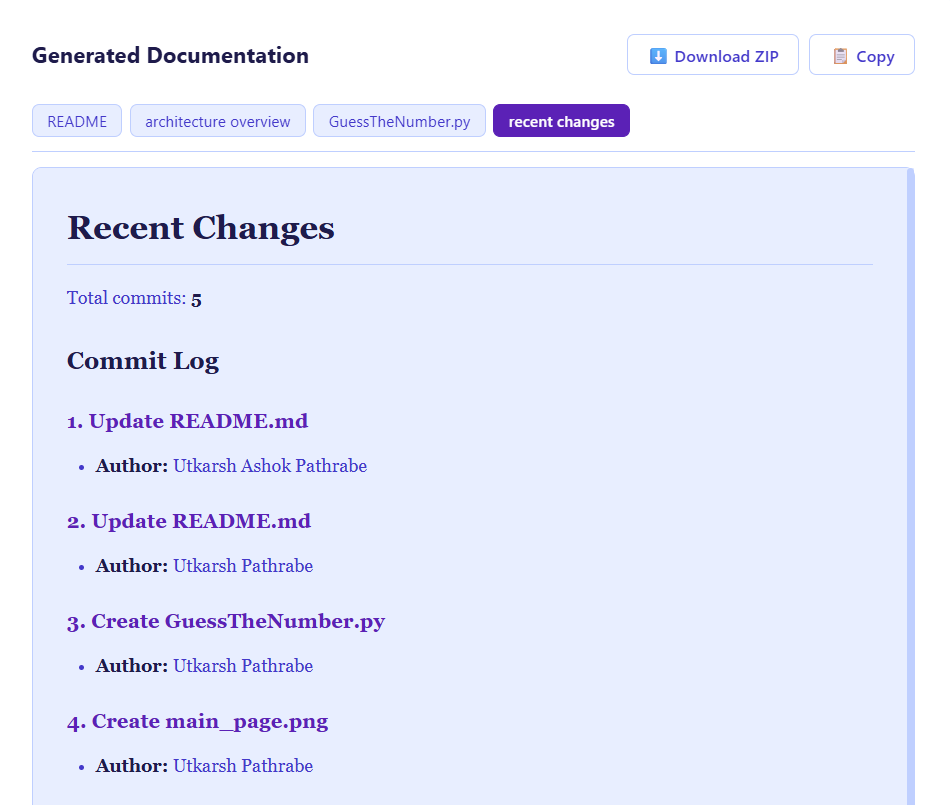
\includegraphics[width=0.6\textwidth]{tex/Screenshot 2026-04-16 073053.png}}
	\caption {recent\_changes.md – Git Commit History Output.}
	\label{lvmh2}
\end{figure}
\FloatBarrier

\section{Discussion}
\hspace{0.5cm}
The results show that the proposed system can efficiently produce overall documentation on different levels, including projects, architecture and functions. The accuracy in the extraction of structural information is guaranteed by AST-based analysis, while graph-based analysis allows for precise identification of relationships between functions. The inclusion of text-based metrics improves the results produced by the system, enhancing their overall relevance and readability.

\par The system works effectively with different programming languages, thus demonstrating the flexibility of the tool. This is further evidenced by the repository URL mode, which is beneficial since the entire projects can be analyzed without the need for file handling. Furthermore, the inclusion of the history of commits is advantageous since it provides additional information compared to other documentation tools.

\par However, the system is not without certain limitations. The quality of the code fed into the system will affect the quality of the documentation that is created. Also, the dynamic behavior of the code is not fully taken into consideration in the system. Nevertheless, the system is useful in reducing the effort required in understanding the code.

% The following figure shows the evaluation of reference audio and test audio by aligning note sequences of both. The green-colored notes represent correct notes. The blue-colored notes are the notes in reference audio missed by test audio. The red-colored notes represent the wrong notes in the test audio. 
% \vspace{1cm}
% \FloatBarrier
% \begin{figure}[h]
% 	\centering
% 	\fbox{\includegraphics[scale=.27]{image/r6.png}}
% 	\caption{Evaluated Notes sequences}
% 	\label{lvmh2}
% \end{figure}
% \FloatBarrier
% % In the following figure show the play back of audio piece correspond to the selected note sequence part. the yellow colored notes are selected by user  for playback. when click  on it a play button is displayed. by click play button the play back can be done.
% %  \vspace{1cm}
% % \FloatBarrier
% % \begin{figure}[h]
% % 	\centering
% % 	\fbox{\includegraphics[scale=.27]{image/result7.png}}
% % 	\caption{Result 7}
% % 	\label{lvmh2}
% % \end{figure}
% % \FloatBarrier
% In the following figure, two play buttons are displayed to playback audio of selected note sequence pieces.
% \vspace{1cm}
% \FloatBarrier
% \begin{figure}[h]
% 	\centering
% 	\fbox{\includegraphics[scale=.27]{image/r7.png}}
% 	\caption{display play buttons on select note sequence peice}
% 	\label{lvmh2}
% \end{figure}
% \FloatBarrier

% % \vspace{1cm}
% % \FloatBarrier
% % \begin{figure}[h]
% % 	\centering
% % 	\fbox{\includegraphics[scale=.27]{image/r8.png}}
% % 	\caption{play back of reference audio}
% % 	\label{lvmh2}
% % \end{figure}
% \FloatBarrier
% The following figure demonstrates inputting reference audio by recording audio using the record button displayed on the interface. Similarly, the test audio can also be recorded in the same manner.
% \vspace{1cm}
% \FloatBarrier
% \begin{figure}[h]
% 	\centering
% 	\fbox{\includegraphics[scale=.27]{image/r9.png}}
% 	\caption{Record reference audio}
% 	\label{lvmh2}
% \end{figure}
% \FloatBarrier

% %  \vspace{1cm}
% % \FloatBarrier
% % \begin{figure}[h]
% % 	\centering
% % 	\fbox{\includegraphics[scale=.27]{image/r10.png}}
% % 	\caption{Record Test audio}
% % 	\label{lvmh2}
% % \end{figure}
% % \FloatBarrier

% % \vspace{1cm}
% % \FloatBarrier
% % \begin{figure}[h]
% % 	\centering
% % 	\fbox{\includegraphics[scale=.27]{image/r11.png}}
% % 	\caption{Note sequence alignment of audio recordings}
% % 	\label{lvmh2}
% % \end{figure}
% % \FloatBarrier
% The following figure shows the time details of notes from audio inputs. 
% \vspace{1cm}
% \FloatBarrier
% \begin{figure}[h]
% 	\centering
% 	\fbox{\includegraphics[scale=.27]{image/r12.png}}
% 	\caption{Display note time sequence}
% 	\label{lvmh2}
% \end{figure}
% \FloatBarrier
% The following figure shows the time duration details of notes and alignment between note sequences from audio inputs.
% \vspace{1cm}
% \FloatBarrier
% \begin{figure}[h]
% 	\centering
% 	\fbox{\includegraphics[scale=.27]{image/r13.png}}
% 	\caption{Display aligned note time sequence}
% 	\label{lvmh2}
% \end{figure}
% \FloatBarrier
% The following figure shows the alignment between note sequences by removing time duration from audio inputs.
%  \vspace{1cm}
% \FloatBarrier
% \begin{figure}[h]
% 	\centering
% 	\fbox{\includegraphics[scale=.27]{image/r14.png}}
% 	\caption{Display aligned note sequence}
% 	\label{lvmh2}
% \end{figure}
% \FloatBarrier
% \subsection{Accuracy in note sequence detection}
% The table below illustrates the accuracy of note sequence detection across various guitar audio recordings.
% \begin{table}[h]
%     \centering
%     \begin{tabular}{|c|c|c|c|}
%         \hline
%          \multirow{2}{*}{}  & Actual note & Detected note &   \\
%           & sequence & sequence & Match \\ 
%         % \thead{ } & \thead{Pitch, onset,\\ & and offset}  & \thead{Pitch and onset} & \thead{Onset only} & \thead{Offset only} \\
%         \hline
%         Guitar Audio 1 & M4 n4	D4	n4 P4 G4 & M4 n4	D4	n4 P4 G4 & \\
%         & D4	P4 M4	D4	M4 & D4	P4 M4	D4	M4 & 100\%\\
%         \hline
%          Guitar Audio 2 & M4 S5	N4	S5 D4   & M4 S5	N4	S5 D4 & \\
%         & N4 D4 M4 D4 P4 & N4 D4 M4 D4 P4 & \\
%          &  M4 G4 P4 & M4 G4 P4 & 100\%\\
%         \hline
%          Guitar Audio 3 & G4	 g4 G4 g4 m4    & G4	 g4 G4 g4 m4 & \\
%         & g4 m4 g4 m4 d4 & g4 m4 g4 m4 d4 & \\
%          &  D4 m4 g4  & D4 m4 g4 & 100\%\\
%         \hline
%          Guitar Audio 4 & d4 n4	D4	p4 P4 & d4 n4	D4	p4 P4 & \\
%         & g4	P4 M4 r4	M4 & g4	P4 M4 r4	M4 & 100\%\\
%         \hline
%          Guitar Audio 5 & s4 r4	G4	m4 P4  & s4 r4	G4	m4 P4 & \\
%           & m4 n4	G4	r4 G4  & m4 n4	G4	r4 G4 & \\
%         & D4 P4 M4	G4	r4 &  D4 P4 M4	G4	r4 & 100\%\\
%         \hline
%     \end{tabular}
%     \caption{Accuracy in detected note sequence of guitar music}
%     \label{tab:simple_table}
% \end{table}
% The table below illustrates the accuracy of note sequence detection across various piano audio recordings.
% \begin{table}[h]
%     \centering
%     \begin{tabular}{|c|c|c|c|}
%         \hline
%          \multirow{2}{*}{}  & Actual note & Detected note &   \\
%           & sequence & sequence & Match \\ 
%         % \thead{ } & \thead{Pitch, onset,\\ & and offset}  & \thead{Pitch and onset} & \thead{Onset only} & \thead{Offset only} \\
%         \hline
%         Guitar Audio 1 & M4 n4	D4	n4 P4 G4 & M4 n4	D4	n4 P4 G4 & \\
%         & D4	P4 M4	D4	M4 & D4	P4 M4	D4	M4 & 100\%\\
%         \hline
%          Guitar Audio 2 & M4 S5	N4	S5 D4   & M4 S5	N4	S5 D4 & \\
%         & N4 D4 M4 D4 P4 & N4 D4 M4 D4 P4 & \\
%          &  M4 G4 P4 & M4 G4 P4 & 100\%\\
%         \hline
%          Guitar Audio 3 & G4	 g4 G4 g4 m4    & G4	 g4 G4 g4 m4 & \\
%         & g4 m4 g4 m4 d4 & g4 m4 g4 m4 d4 & \\
%          &  D4 m4 g4  & D4 m4 g4 & 100\%\\
%         \hline
%          Guitar Audio 4 & d4 n4	D4	p4 P4 & d4 n4	D4	p4 P4 & \\
%         & g4	P4 M4 r4	M4 & g4	P4 M4 r4	M4 & 100\%\\
%         \hline
%          Guitar Audio 5 & s4 r4	G4	m4 P4  & s4 r4	G4	m4 P4 & \\
%           & m4 n4	G4	r4 G4  & m4 n4	G4	r4 G4 & \\
%         & D4 P4 M4	G4	r4 & D4 P4 M4	G4	r4 & 100\%\\
%         \hline
%     \end{tabular}
%     \caption{Accuracy in detected note sequence of piano music}
%     \label{tab:simple_table}
% \end{table}
%  To assess the accuracy of note sequences, several piano and guitar audio recordings were examined, revealing a 100\% accuracy rate. However, identifying the actual note sequence in vocal audio poses challenges due to variations in voice tone. But we can expect the note sequence of vocal audio. Here, the detected note sequence is also evaluated based on the expected note sequence. It provides accuracy of more than 80\% in vocal audio note sequence detection. If the audio is noise-free then it can provide 100\% accuracy. The proposed system can be used only for monophonic audio.
%  \subsection{ Result of Note sequence alignment}
%  The proposed Dynamic Time Warping algorithm has optimally aligned the note sequence, obtaining the maximum matching between note sequences. It accurately shows mistakes in test notes and provides a match score. Since the Dynamic Time Warping algorithm uses dynamic programming, its accuracy is 100\%.
% \par
% Figure 7.1 depicts the home page of the application. On the left side of the page, there are three buttons, while a frame is positioned on the right. The content within the frame dynamically changes according to the buttons clicked on the left side of the page. The first button name with \textbf{Create Tune} navigates to the tune creation process, the second button name with \textbf{Play Tune} leads to the tune playback process, and the third button name with \textbf{Convert to audio} directs to the audio conversion process.  
% \FloatBarrier
% \begin{figure}[h]
% 	\centering
% 	\fbox{\includegraphics[scale=.26]{image/result3.png}}
% 	\caption{Raga Selection}
% 	\label{lvmh2}
% \end{figure}
% \FloatBarrier

% Figure 7.2 shows the raga selection process initiated upon clicking the \textbf{Create Tune} button. It displays 72 raga options for selection. Upon choosing a raga, the interface navigates to another page, as represented in Figure 7.3. 



% \FloatBarrier
% \begin{figure}[h]
% 	\centering
% 	\fbox{\includegraphics[scale=.26]{image/result5.png}}
% 	\caption{Virtual Keyboard}
% \end{figure}
% \FloatBarrier

% \par Figure 7.3 demonstrates the presentation of a virtual keyboard corresponding to the selected raga. Each key on the virtual keyboard is associated with microtones of notes, concurrently mapped with the system keyboard labeled from 1 to 9. This interface enables the creation of note sequences. Additionally, this page offers options to customize instrument sounds, a button for tune replay, a slider to adjust speed, as well as buttons to save or discard tunes. When the 'Save' button is clicked, it prompts the user to enter a file name.

% \FloatBarrier
% \begin{figure}[h]
% 	\centering
% 	\fbox{\includegraphics[scale=.26]{image/result7.png}}
% 	\caption{Playback Tune}
% \end{figure}
% \FloatBarrier

% \par Figure 7.4 demonstrates the tune-playing process initiated upon clicking the \textbf{Play Tune} button. This interface provides an input feature to upload a sequence file to play and offers options to customize instrument sounds, a button for tune play, and a slider to adjust speed.

% \FloatBarrier
% \begin{figure}[h]
% 	\centering
% 	\fbox{\includegraphics[scale=.26]{image/result9.png}}
% 	\caption{Input sequence file for audio conversion}
% \end{figure}
% \FloatBarrier
% % \par In figure 7.5, the same person's ECG is taken in a different date.

% % \FloatBarrier
% % \begin{figure}[h]
% % 	\centering
% % 	\fbox{\includegraphics[scale=.27]{image/result11.png}}
% % 	\caption{Sample Output 2}
% % \end{figure}
% % \FloatBarrier
% \par Figure 7.5 demonstrates the audio converting process initiated upon clicking the \textbf{Convert to Audio} button. This interface provides an input feature to upload a sequence file to convert into audio and offers options to customize instrument sounds, a button name with \textbf{Make Audio file}, and a slider to adjust speed. Upon clicking the \textbf{Make Audio file} button, the interface navigates to another page, as represented in Figure 7.6. 
% \FloatBarrier

% \begin{figure}[h]
% 	\centering
% 	\fbox{\includegraphics[scale=.26]{image/result10.png}}
% 	\caption{sequence file to audio conversion}
% \end{figure}
% \FloatBarrier
% \par Figure 7.6 illustrates the outcome after clicking the \textbf{Make Audio file} button. The  \textbf{Play} button enables previewing of the converted audio, and the  \textbf{Download} button allows users to download it. Upon clicking the \textbf{Download} button, the interface prompts the user to enter a file name, as represented in Figure 7.7. 

% \FloatBarrier
% \begin{figure}[h]
% 	\centering
% 	\fbox{\includegraphics[scale=.26]{image/result12.png}}
% 	\caption{Downloading audiofile}
% \end{figure}
% \FloatBarrier
% \textbf{Result:} All the functionalities provided in the system, such as raga selection, instrument selection, playback speed adjustment, playing tunes from sequence files, and audio conversion, are operating smoothly. The tune played from the sequence file achieves a 100\% accuracy rate. The audio obtained after converting the sequence file to an audio file precisely matches the played tune.

% \chapter{Evaluation and Results}

%\section{Performance Evaluation}
% \subsection{Evaluation Result}

% \subsubsection{Field Extraction Accuracy}
% Field extraction was carried out using a combination of libraries such as \texttt{pdfplumber} for digital PDFs and \texttt{pytesseract} with preprocessing techniques (binarization, noise removal, thresholding) for scanned images. The extracted text was cleaned and normalized using regular expressions and \texttt{numpy}.  

% For digital PDFs, the system extracted most fields accurately. Aadhaar numbers from Digilocker PDFs appeared masked (e.g., \texttt{XXXX XXXX 1234}), and Driving License numbers were extracted correctly but without spacing between the regional code and number (e.g., \texttt{KL089875678229} instead of \texttt{KL08 9875678229}). In rare cases (1 out of 8), the Aadhaar Name field concatenated with the address label due to formatting inconsistencies. Other fields such as Date of Birth, Gender, Address, SGPA, and Percentage were extracted with full accuracy.  

% When a scanned Aadhaar image (JPEG) was uploaded in addition to the PDFs, the full Aadhaar number was extracted successfully, and the Name concatenation issue was avoided, improving overall accuracy.  

% % \begin{table}[H]
% % \centering
% % \caption{Field-wise Accuracy (PDFs only)}
% % \begin{tabular}{|l|c|l|}
% % \hline
% % \textbf{Field} & \textbf{Accuracy} & \textbf{Remarks} \\ \hline
% % Name & 87--88\% & Correct in most cases. \\ \hline
% % Date of Birth & 100\% & Consistently extracted. \\ \hline
% % Gender & 100\% & Extracted from Aadhaar. \\ \hline
% % Aadhaar Number & 50\% & Masked in Digilocker PDFs  \\ \hline
% % PAN Number & 100\% & Fully extracted. \\ \hline
% % Driving License Number & $\sim$95\% & Value correct; spacing issue present. \\ \hline
% % Address & 100\% & Extracted reliably. \\ \hline
% % SGPA & 100\% & Extracted from marklists. \\ \hline
% % Percentage & 100\% & Extracted from marklists. \\ \hline
% % \end{tabular}
% % \end{table}

% \noindent Overall field extraction accuracy with only PDFs was approximately \textbf{88--90\%}, with main limitations being the masked Aadhaar number, minor formatting inconsistencies in Driving License numbers, and rare concatenation of Aadh-aar Name with Address.
% \subsection{Field Extraction Accuracy}
% \hspace{0.5cm} Field extraction used \texttt{pdfplumber} for digital PDFs and \texttt{pytesseract} with preprocessing (binarization, noise removal, thresholding) for scanned images. Text was cleaned and normalized with regular expressions and \texttt{numpy}.  

% Most fields were accurately extracted from PDFs. Aadhaar numbers from Digilocker PDFs were masked (e.g., \texttt{XXXX XXXX 1234}) and Driving License numbers lacked spacing (e.g., \texttt{KL089875678229}). Rarely, the Aadhaar Name concatenated with the address. Other fields, including Date of Birth, Gender, Address, SGPA, and Percentage, were fully extracted.  

% Adding scanned Aadhaar images resolved masking and concatenation issues. Overall field extraction accuracy with PDFs alone was around \textbf{88--90\%}, with minor limitations due to masked Aadhaar numbers and formatting inconsistencies.



% \subsection{Consolidated Profile Accuracy}
% \hspace{0.3cm} The consolidation step merged extracted fields from multiple documents into a unified profile. Conflicts (e.g., different spellings of a name or minor formatting differences) were resolved using frequency-based selection and semantic similarity matching with \texttt{sentence-transformers}.  
% Across all tested cases, the system achieved \textbf{100\% consolidation accuracy}, producing reliable profiles.

% \subsection{Form Auto-Filling Accuracy}
% \hspace{0.3cm} For form filling, extracted fields were mapped to target form fields using semantic similarity techniques. Even when labels in the form were phrased differently (e.g., ``DOB'' vs ``Date of Birth''), the model correctly identified matches. The auto-fill module then populated the fields using Python browser automation.  
% In testing with 16 expected form fields, the system filled all fields correctly, resulting in a \textbf{100\% form filling accuracy}.

% \subsection{User Verification and Correction Rate}
% \hspace{0.3cm} Once the form was auto-filled, users could review the results. Since the system’s accuracy was very high, manual corrections were rarely required. For digital PDFs alone, Aadhaar numbers required correction due to masking, and the occasional Name concatenation had to be fixed. With supporting Aadhaar images provided, no manual corrections were necessary, except for minor adjustments in the Driving License number formatting.  
% This gives the system an effective correction rate of \textbf{0--2\%}, showing strong reliability.

% \subsubsection{Processing Time}
% The system processed digital PDFs efficiently, completing extraction and form filling in an average of \textbf{3--5 seconds} for four documents. When scanned images were included, the time increased slightly due to OCR preprocessing, averaging \textbf{5--7 seconds}, which is still acceptable for practical use. 
% \subsection{Processing Time}
% \hspace{0.3cm} The system processed digital PDFs efficiently, completing extraction and form filling in an average of \textbf{3--5 seconds} for four documents. When scanned images were included, the time increased slightly due to OCR preprocessing, averaging \textbf{5--7 seconds}. These times were measured by recording the duration from the moment documents were uploaded to the point when the form was fully autofilled, using Python's built-in timing functions, which provides a practical estimate of real-world performance.

% \newpage
% \subsection{Observations}
% \begin{itemize}
%     \item Digital PDFs achieved high accuracy, but Aadhaar numbers were masked in Digilocker files.
%     \item In 1 of 8 cases, the Aadhaar Name field concatenated with the Address, slightly reducing accuracy.
%     \item Adding scanned Aadhaar images resolved masking and name concat-enation, improving accuracy to nearly 100\%.
%     \item Driving License numbers were correct but spacing inconsistencies slightly reduced accuracy.
%     \item The auto-filling module demonstrated robustness by correctly mapping fields even with inconsistent naming.
%     \item Minimal user corrections were required, confirming the system’s efficie-ncy and practicality.
% \end{itemize}

% \subsection*{\hspace{-0.1cm}Observations}
% \begin{itemize}
%     \item Digital PDFs were generally accurate, though Aadhaar numbers were masked.
%     \item Rarely, Aadhaar Name concatenated with the Address, slightly reducing accuracy.
%     \item Adding scanned Aadhaar images resolved masking and concatenation issues.
%     \item Driving License numbers had minor spacing inconsistencies.
%     \item Auto-filling correctly mapped fields even with inconsistent naming.
%     \item Minimal user corrections were needed, confirming system reliability.
% \end{itemize}

%\chapter{CONCLUSION}

\hspace{0.5cm} The proposed AI-Powered Code Document Generator would thus offer an intelligent and automated solution for the generation of accurate, structured, and context-aware documentation from source code. This would thus help in the identification of significant software components like functions, classes, imports, call relationships, entry points, and recursive patterns, among others. In this regard, the proposed solution would leverage Tree-sitter for parsing code across fourteen programming languages and thus generate accurate documentation like the README file, architecture, description of files, recent changes of the git repository, among others.

\par The system relies on a three-stage feature extraction process to guarantee the LLM access to rich and non-redundant information for every function it documents. Features extracted from the AST offer structural information such as the function’s name, class membership, parameters, return type, and calls. Features extracted from the text offer context-based information on the file’s complexity and documentation. Features extracted from the graph offer architectural information on the function and the program based on the NetworkX library’s directed call graph. By combining all the features in a single fact block, the system offers documentation that is functionally correct, contextually scaled and architecturally aware.

\par This modular and language-independent design ensures that each module is independent in its functioning through well-defined interfaces. It is possible to upgrade or extend any module in the pipeline without affecting the rest of the pipeline. Cross-file awareness ensures that functions used across module boundaries are correctly identified as active rather than unused, thereby improving the reliability of the architectural analysis. The parallel document generation using the \texttt{ThreadPoolExecutor} ensures the pipeline scales well with projects of different sizes.

\par This tool is highly beneficial for software development teams working with repositories that lack adequate documentation. It boosts productivity by automating what is usually a manual and time-consuming process. Additionally, it supports long-term code maintainability by allowing developers to understand the code’s structure through graph-based analysis.

\par Overall, the project highlights the potential of combining artificial intelligence with static code analysis to create a practical tool that simplifies software documentation. Future improvements could include extending support to more programming languages, integrating with version control systems to enable real-time documentation updates and employing more advanced language models for richer, more detailed explanations, ultimately developing the system into a comprehensive, production-ready documentation platform.
\newline
\par Despite the current system addressing many key challenges in automated documentation, there is room for improvement by enhancing system capabilities, supporting additional programming languages and adding new features to make the system more intelligent and adaptive. These opportunities pave the way for future developments that could increase the system’s effectiveness and applicability in real-world software development scenarios which discussed in next chapter.
%\chapter{FUTURE ENHANCEMENT}

\hspace{0.5cm} The AI-Powered Code Document Generator sets a robust foundation for automated documentation, demonstrating how static code analysis and large language models can work together to produce accurate, structured and context-rich documentation for multiple programming languages. This chapter explores several opportunities for enhancing and refining the system to advance it toward a more comprehensive, production-ready platform.

\section{Git Integration}
\hspace{0.5cm} One of the way to improve the system would be to integrate it more closely with Git-based platforms like GitHub and GitLab. Currently, documentation is generated when a user provides a repository URL or manually uploads files. Enhanced Git integration could allow the documentation to update automatically with each commit.



\section{Multi-Language Expansion}
\hspace{0.5cm} Although the system currently supports fourteen programming languages, future upgrades could add support for languages like Swift, Scala, Dart and Haskell. Expanding language compatibility would make the system applicable to a wider range of development projects beyond its current scope.


\section{Interactive Q\&A}
\hspace{0.5cm} A highly valuable future feature could be the addition of an intelligent Question\&Answer system (Q\&A ), allowing developers to interact with the codebase through a natural language interface. Instead of merely reviewing the automatically generated documentation, developers could directly ask questions about function call chains, recent changes or other specific aspects of the system.


\newline
\hspace{0.5cm}The future improvements proposed in this chapter represent a natural progression of the current system. Git integration would embed documentation generation into the ongoing development workflow. Expanding multi-language support would broaden the system’s applicability across diverse programming environments. Adding an interactive Q\&A feature would transform the system from a passive documentation generator into an active tool for code understanding. Collectively, these enhancements would result in a highly efficient and practical automated documentation platform.
%\input{tex/bibliography}
%\input{tex/annexure}


\newpage
\begin{thebibliography}{10}

\bibitem{Song2024}
J. Song, Z. Zhang, Z. Tang, S. Feng, and Y. Gu,
``Improving Code Summarization With Tree Transformer Enhanced by Position-Related Syntax Complement,''
\emph{IEEE Transactions on Artificial Intelligence}, vol. 5, no. 9, pp. 4776--478X, Sept. 2024, doi: 10.1109/TAI.2024.3395231.
\bibitem{Rozi2023}
M. F. Rozi, T. Ban, S. Ozawa, A. Yamada, T. Takahashi, S. Kim, and D. Inoue,
``Detecting Malicious JavaScript Using Structure-Based Analysis of Graph Representation,''
\emph{IEEE Access}, vol. 11, pp. 102727--1027XX, 2023, doi: 10.1109/ACCESS.2023.3317266.

\bibitem{Mostafavi2024}
M. M. Ghahfarokhi, A. Khademian, S. Kianiangolafshani, A. Asadi, H. Jahantigh, and A. Heydarnoori,
``Beyond Syntax: Unleashing the Power of Computational Notebooks Code Metrics in Documentation Generation,''
in \emph{Proc. IEEE/ACM Int. Conf. AI Engineering -- Software Engineering for AI (CAIN)}, Lisbon, Portugal, Apr. 2024, pp. 278--280, doi: 10.1145/3644815.3644979.

\bibitem{Wang2020}
W. Wang, Y. Zhang, Y. Sui, Y. Wan, Z. Zhao, J. Wu, P. S. Yu, and G. Xu,
``Reinforcement-Learning-Guided Source Code Summarization using Hierarchical Attention,''
\emph{IEEE Transactions on Software Engineering}, 2020.
\bibitem{CodeDocAgent2025}
S. Yao, Y. Shen, D. Liu, and J. Hu,
``CodeDocAgent: Leveraging Large Language Models for Accurate and Contextual Code Documentation,''
in \emph{Proceedings of IEEE}, 2025.

\bibitem{Zhu2025}
Y. Zhu, X. Zhao, X. Li, Y. Zou, H. Yuan, Y. Wang, and B. Xie,
``RepoSummary: Feature-Oriented Summarization and Documentation Generation for Code Repositories,''
in \emph{Proc. ACM Conf.}, 2025.

\bibitem{KhanUddin2023}
J. Y. Khan and G. Uddin,
``Combining Contexts from Multiple Sources for Documentation-Specific Code Example Generation,''
in \emph{Proc. IEEE Int. Conf. Software Analysis, Evolution and Reengineering (SANER)}, 2023, pp. 683--693, doi: 10.1109/SANER56733.2023.00071.

\bibitem{Thota2024}
S. R. Thota, S. Arora, and S. Gupta,
``AI-Driven Automated Software Documentation Generation for Enhanced Development Productivity,''
in \emph{Proc. Int. Conf. Data Science and Network Security (ICDSNS)}, 2024.

\bibitem{GhaleDabbagh2025}
D. P. Ghale and M. Dabbagh,
``Automated Code Comments Generation Using Large Language Models: Empirical Evaluation of T5 and BART,''
\emph{IEEE Access}, vol. 13, pp. 141420--1414XX, 2025, doi: 10.1109/ACCESS.2025.3597601.

\bibitem{Procko2023}
T. T. Procko and S. Collins, ``Automatic Code Documentation with Syntax Trees and GPT: Alleviating Software Development’s Most Redundant Task,'' Embry-Riddle Aeronautical University, Daytona Beach, FL, USA.

\end{thebibliography}

\addcontentsline{toc}{chapter}{Bibliography}
% \bibliographystyle{unsrt}
% %\pagestyle{plain}
% \bibliography{bib/thesis}

\end{spacing}

\end{document}
